% Result values are macros from numbers.tex; tables/ and figures/ are generated from the stored results by
% build_displays.py, and refs.bib by make_bib.py. build_pdf.py compiles the named and the anonymous version.
\documentclass[11pt]{article}
\usepackage[margin=1in]{geometry}
\usepackage[T1]{fontenc}
\usepackage[utf8]{inputenc}
\usepackage{lmodern,microtype}
\usepackage{booktabs,graphicx,amsmath,amssymb,array,tabularx}
\usepackage{xcolor,enumitem,caption,placeins,adjustbox,etoolbox}
\usepackage[numbers,sort&compress]{natbib}
\usepackage[hidelinks]{hyperref}
\usepackage{xurl}
% Generated by manuscript/make_numbers.py from logged results. Do not edit by hand.
\newcommand{\ContainFixedCuad}{91.1}
\newcommand{\ContainFixedQasper}{75.5}
\newcommand{\ContainParagraphCuad}{99.0}
\newcommand{\ContainParagraphQasper}{98.6}
\newcommand{\ContainSentenceCuad}{99.3}
\newcommand{\ContainSentenceQasper}{80.8}
\newcommand{\EoneNq}{9,253}
\newcommand{\EoneNqCovidqa}{1,771}
\newcommand{\EoneNqCuad}{996}
\newcommand{\EoneNqQasper}{1,742}
\newcommand{\EoneNqSquadtwo}{4,744}
\newcommand{\EtwoEmFiveTwelveBudget}{0.125}
\newcommand{\EtwoEmFiveTwelveCount}{0.090}
\newcommand{\EtwoEmOneTwoEightBudget}{0.085}
\newcommand{\EtwoEmOneTwoEightCount}{0.105}
\newcommand{\EtwoJobsCuad}{400}
\newcommand{\EtwoJobsQasper}{400}
\newcommand{\EtwoPoneCov}{+0.089}
\newcommand{\EtwoPoneCovHi}{+0.132}
\newcommand{\EtwoPoneCovLo}{+0.050}
\newcommand{\EtwoPoneCovMde}{0.059}
\newcommand{\EtwoPoneEm}{\ensuremath{-}0.055}
\newcommand{\EtwoPoneEmCovid}{\ensuremath{-}0.060}
\newcommand{\EtwoPoneEmDoc}{\ensuremath{-}0.055}
\newcommand{\EtwoPoneEmDocHi}{\ensuremath{-}0.020}
\newcommand{\EtwoPoneEmDocLo}{\ensuremath{-}0.095}
\newcommand{\EtwoPoneEmHi}{\ensuremath{-}0.010}
\newcommand{\EtwoPoneEmLo}{\ensuremath{-}0.100}
\newcommand{\EtwoPoneEmMde}{0.066}
\newcommand{\EtwoPoneEmSquad}{\ensuremath{-}0.160}
\newcommand{\EtwoPoneEmUntrunc}{\ensuremath{-}0.055}
\newcommand{\EtwoPoneEmUntruncHi}{\ensuremath{-}0.010}
\newcommand{\EtwoPoneEmUntruncLo}{\ensuremath{-}0.105}
\newcommand{\EtwoPoneFone}{\ensuremath{-}0.017}
\newcommand{\EtwoPoneFoneHi}{+0.033}
\newcommand{\EtwoPoneFoneLo}{\ensuremath{-}0.065}
\newcommand{\EtwoPoneFoneMde}{0.068}
\newcommand{\EtwoPoneFoneMdeStrat}{0.068}
\newcommand{\EtwoSquadFiveTwelveBudgetCov}{0.88}
\newcommand{\EtwoSquadFiveTwelveBudgetFone}{0.58}
\newcommand{\EtwoSquadOneTwoEightBudgetCov}{0.86}
\newcommand{\EtwoSquadOneTwoEightBudgetFone}{0.44}
\newcommand{\EtwoSthreeCov}{+0.035}
\newcommand{\EtwoSthreeCovHi}{+0.060}
\newcommand{\EtwoSthreeCovLo}{+0.015}
\newcommand{\EtwoSthreeCovMde}{0.036}
\newcommand{\EtwoSthreeEm}{\ensuremath{-}0.015}
\newcommand{\EtwoSthreeEmHi}{+0.020}
\newcommand{\EtwoSthreeEmLo}{\ensuremath{-}0.050}
\newcommand{\EtwoSthreeEmMde}{0.051}
\newcommand{\EtwoSthreeFone}{+0.004}
\newcommand{\EtwoSthreeFoneHi}{+0.036}
\newcommand{\EtwoSthreeFoneLo}{\ensuremath{-}0.024}
\newcommand{\EtwoSthreeFoneMde}{0.044}
\newcommand{\EtwoTruncCuad}{65}
\newcommand{\EtwoTruncQasper}{2}
\newcommand{\EtwoTruncQueriesCuad}{26}
\newcommand{\EtwoTruncQueriesQasper}{2}
\newcommand{\GoldMedianQasper}{72.5}
\newcommand{\HFiveBBudget}{91.7}
\newcommand{\HFiveBCount}{33.3}
\newcommand{\HFiveBDocEst}{58.3}
\newcommand{\HFiveBDocHi}{75.0}
\newcommand{\HFiveBDocLo}{47.9}
\newcommand{\HFiveBDocVerdict}{supported}
\newcommand{\HFiveBEst}{58.3}
\newcommand{\HFiveBHi}{64.6}
\newcommand{\HFiveBLo}{45.1}
\newcommand{\HFiveBPilotBudget}{91.7}
\newcommand{\HFiveBPilotCount}{31.2}
\newcommand{\HFiveBPlannedEst}{58.3}
\newcommand{\HFiveBPlannedHi}{64.6}
\newcommand{\HFiveBPlannedLo}{45.1}
\newcommand{\HFiveBPlannedVerdict}{supported}
\newcommand{\HFiveBVerdict}{supported}
\newcommand{\HFiveBudgetFiveTwelve}{5.6}
\newcommand{\HFiveCountFiveTwelve}{27.1}
\newcommand{\HFiveDocEst}{19.4}
\newcommand{\HFiveDocHi}{39.6}
\newcommand{\HFiveDocLo}{16.7}
\newcommand{\HFiveDocVerdict}{inconclusive}
\newcommand{\HFiveEst}{21.5}
\newcommand{\HFiveHi}{41.7}
\newcommand{\HFiveLo}{16.7}
\newcommand{\HFivePilotCountFiveTwelve}{8.3}
\newcommand{\HFivePlannedEst}{19.4}
\newcommand{\HFivePlannedHi}{41.7}
\newcommand{\HFivePlannedLo}{16.7}
\newcommand{\HFivePlannedVerdict}{inconclusive}
\newcommand{\HFiveReplicateOffset}{5.5}
\newcommand{\HFiveVerdict}{supported}
\newcommand{\HFourBBudget}{72.2}
\newcommand{\HFourBCount}{6.9}
\newcommand{\HFourBDocEst}{65.2}
\newcommand{\HFourBDocHi}{67.1}
\newcommand{\HFourBDocLo}{55.4}
\newcommand{\HFourBDocVerdict}{supported}
\newcommand{\HFourBEst}{65.3}
\newcommand{\HFourBHi}{68.3}
\newcommand{\HFourBLo}{56.5}
\newcommand{\HFourBPlannedEst}{64.4}
\newcommand{\HFourBPlannedHi}{68.3}
\newcommand{\HFourBPlannedLo}{56.5}
\newcommand{\HFourBPlannedVerdict}{supported}
\newcommand{\HFourBVerdict}{supported}
\newcommand{\HFourBmOnlyBudget}{61.1}
\newcommand{\HFourBmOnlyCount}{0.0}
\newcommand{\HFourBmOnlyEst}{61.1}
\newcommand{\HFourBmOnlyHi}{72.5}
\newcommand{\HFourBmOnlyLo}{57.2}
\newcommand{\HFourBudget}{65.3}
\newcommand{\HFourCount}{9.7}
\newcommand{\HFourDenseOnlyBudget}{69.4}
\newcommand{\HFourDenseOnlyCount}{19.4}
\newcommand{\HFourDenseOnlyEst}{50.0}
\newcommand{\HFourDenseOnlyHi}{58.1}
\newcommand{\HFourDenseOnlyLo}{39.1}
\newcommand{\HFourDocEst}{59.0}
\newcommand{\HFourDocHi}{65.0}
\newcommand{\HFourDocLo}{51.3}
\newcommand{\HFourDocVerdict}{supported}
\newcommand{\HFourEst}{55.6}
\newcommand{\HFourHi}{63.1}
\newcommand{\HFourLo}{50.8}
\newcommand{\HFourPlannedEst}{55.4}
\newcommand{\HFourPlannedHi}{63.1}
\newcommand{\HFourPlannedLo}{50.8}
\newcommand{\HFourPlannedVerdict}{supported}
\newcommand{\HFourVerdict}{supported}
\newcommand{\HOneBDocEst}{26.4}
\newcommand{\HOneBDocHi}{34.4}
\newcommand{\HOneBDocLo}{15.0}
\newcommand{\HOneBDocVerdict}{supported}
\newcommand{\HOneBEst}{27.1}
\newcommand{\HOneBHi}{33.9}
\newcommand{\HOneBLo}{15.4}
\newcommand{\HOneBPlannedEst}{26.7}
\newcommand{\HOneBPlannedHi}{33.9}
\newcommand{\HOneBPlannedLo}{15.4}
\newcommand{\HOneBPlannedVerdict}{supported}
\newcommand{\HOneBVerdict}{supported}
\newcommand{\HOneCoverageDecline}{72.7}
\newcommand{\HOneDocEst}{68.9}
\newcommand{\HOneDocHi}{80.9}
\newcommand{\HOneDocLo}{61.6}
\newcommand{\HOneDocVerdict}{supported}
\newcommand{\HOneEst}{70.9}
\newcommand{\HOneHi}{81.9}
\newcommand{\HOneLenientDecline}{70.7}
\newcommand{\HOneLo}{64.8}
\newcommand{\HOnePlannedEst}{71.1}
\newcommand{\HOnePlannedHi}{81.9}
\newcommand{\HOnePlannedLo}{64.8}
\newcommand{\HOnePlannedVerdict}{supported}
\newcommand{\HOneStrictDecline}{69.3}
\newcommand{\HOneVerdict}{supported}
\newcommand{\HThreeMedianN}{1,256}
\newcommand{\HThreeShare}{85.4}
\newcommand{\HThreeVerdict}{supported}
\newcommand{\HTwoDatasetEta}{0.61}
\newcommand{\HTwoDocFraction}{100.0}
\newcommand{\HTwoDocVerdict}{supported}
\newcommand{\HTwoFraction}{100.0}
\newcommand{\HTwoRetrieverEta}{0.04}
\newcommand{\HTwoVerdict}{supported}
\newcommand{\InferenceShiftMax}{2.1}
\newcommand{\PilotBounds}{8}
\newcommand{\PilotMaxDiff}{1.85}
\newcommand{\PoneBudgetFiveTwelve}{7.6}
\newcommand{\PoneBudgetOneTwoEight}{81.2}
\newcommand{\PoneCountFiveTwelve}{78.5}
\newcommand{\PoneCountOneTwoEight}{0.0}
\newcommand{\PoneDenseOneUniverse}{2.1}
\newcommand{\PoneDenseUniversesBudget}{36}
\newcommand{\PoneDenseUniversesCount}{48}
\newcommand{\PoneUniversesBudget}{576}
\newcommand{\PoneUniversesCount}{768}
\newcommand{\PosthocCharFlips}{965}
\newcommand{\PosthocEquivElements}{85,275,648}
\newcommand{\PosthocEquivElementsB}{1,665,540}
\newcommand{\PosthocUniverses}{24,960}
\newcommand{\QasperContainedDelta}{0.015}
\newcommand{\QasperSplitDelta}{0.075}
\newcommand{\QasperSplitShare}{24.5}
\newcommand{\QasperStrictBudgetFiveTwelve}{91.7}
\newcommand{\QasperStrictBudgetOneTwoEight}{0.0}
\newcommand{\ReplicateOffsetMax}{6.3}
\newcommand{\SemBpMax}{320}
\newcommand{\SemBpMin}{278}
\newcommand{\SemClMax}{458}
\newcommand{\SemClMin}{452}
\newcommand{\SemClNoncontigMin}{92.0}
\newcommand{\SensAllBudgetsEst}{73.9}
\newcommand{\SensAllBudgetsHi}{84.8}
\newcommand{\SensAllBudgetsLo}{68.3}
\newcommand{\SensBHEst}{67.6}
\newcommand{\SensBHPooledEst}{70.2}
\newcommand{\SensClusterEst}{68.9}
\newcommand{\SensClusterHi}{80.9}
\newcommand{\SensClusterLo}{61.6}
\newcommand{\SensDefRetEst}{70.8}
\newcommand{\SensDefRetHi}{85.4}
\newcommand{\SensDefRetLo}{64.6}
\newcommand{\SensNoSquadEst}{61.2}
\newcommand{\SensNoSquadHi}{74.8}
\newcommand{\SensNoSquadLo}{53.2}
\newcommand{\SfiveOneTwoEightBudgetFix}{75.0}
\newcommand{\SfiveOneTwoEightBudgetSem}{8.3}
\newcommand{\SfiveOneTwoEightCountFix}{16.7}
\newcommand{\SfiveOneTwoEightCountSem}{60.4}
\newcommand{\SfiveUniversesBudget}{72}
\newcommand{\SfiveUniversesCount}{96}
\newcommand{\SoneOneTwoEightBudgetA}{60.8}
\newcommand{\SoneOneTwoEightBudgetB}{6.5}
\newcommand{\SoneOneTwoEightCountA}{0.0}
\newcommand{\SoneOneTwoEightCountB}{75.4}
\newcommand{\SoneSixFourBudgetA}{20.0}
\newcommand{\SoneSixFourBudgetB}{42.5}
\newcommand{\SoneSixFourCountB}{83.9}
\newcommand{\SquadContainedDelta}{0.033}
\newcommand{\SquadSplitN}{23}
\newcommand{\StwoOneTwoEightBudgetA}{54.8}
\newcommand{\StwoOneTwoEightBudgetB}{1.9}
\newcommand{\StwoOneTwoEightCountA}{52.0}
\newcommand{\StwoOneTwoEightCountB}{1.8}
\newcommand{\StwoTwoFiveSixBudgetA}{39.8}
\newcommand{\StwoTwoFiveSixBudgetB}{2.9}
\newcommand{\StwoTwoFiveSixCountA}{36.2}
\newcommand{\StwoTwoFiveSixCountB}{3.3}
\newcommand{\UnderfillCells}{2}
\newcommand{\UnderfillMaxShift}{0.1}
\newcommand{\UnderfillWordsA}{1,880}
\newcommand{\UnderfillWordsB}{1,789}

\newcommand{\pp}{\ensuremath{\,\mathrm{pp}}}
\newcommand{\chunk}[1]{\texttt{#1}}
\newcommand{\ind}{\mathbb{1}}
\providecommand{\AnonymousSubmission}{0}
\ifnum\AnonymousSubmission=1
  \newcommand*{\AuthorName}{}
\else
  \newcommand*{\AuthorName}{Swaroop Chand J C}
\fi
\newcommand*{\AuthorAffiliation}{}
\newcommand*{\AuthorEmail}{}
\captionsetup{font=small,labelfont=bf,skip=6pt}
\setlength{\emergencystretch}{2em}
\setlength{\tabcolsep}{3pt}
\setlist{nosep}
\renewcommand{\bibfont}{\small}
\setlength{\bibsep}{3pt}
\renewcommand{\topfraction}{0.92}
\renewcommand{\bottomfraction}{0.85}
\renewcommand{\textfraction}{0.08}
\renewcommand{\floatpagefraction}{0.75}
\setcounter{topnumber}{3}
\setcounter{totalnumber}{5}
% Fit generated tables without editing their numerical contents or filenames.
\BeforeBeginEnvironment{tabular}{\begin{adjustbox}{max width=\linewidth}}
\AfterEndEnvironment{tabular}{\end{adjustbox}}
% Let generated [t] tables also float here in this single-column layout.
\let\RepoTable\table
\let\EndRepoTable\endtable
\renewenvironment{table}[1][htbp]{\RepoTable[htbp]}{\EndRepoTable}
\renewenvironment{table*}[1][htbp]{\RepoTable[htbp]}{\EndRepoTable}

\hypersetup{pdftitle={Chunking Verdicts in Retrieval-Augmented Generation Depend on the Evaluation Protocol: A Multiverse Analysis},pdfsubject={Multiverse analysis of chunking evaluation protocols},pdfauthor={\AuthorName}}
\title{Chunking Verdicts in Retrieval-Augmented Generation Depend on the Evaluation Protocol:\texorpdfstring{\\}{ }A Multiverse Analysis}
\author{\AuthorName}
\date{}
\makeatletter
\renewcommand{\@maketitle}{%
  \begin{center}
    {\LARGE \@title\par}
    \ifx\AuthorName\@empty\else
      \vskip 0.8em {\large \AuthorName\par}
      \ifx\AuthorAffiliation\@empty\else\AuthorAffiliation\par\fi
      \ifx\AuthorEmail\@empty\else\texttt{\AuthorEmail}\par\fi
    \fi
  \end{center}
  \vskip 0.8em
}
\makeatother
\begin{document}
\maketitle

\begin{abstract}
Studies that compare chunking strategies for retrieval-augmented generation often retrieve a fixed number of chunks, so longer chunks also bring more text. Under evidence-coverage metrics, that extra text can look like better segmentation. We measure how much this matters with a multiverse analysis over four English question-answering datasets (\EoneNq{} held-out queries), scoring word-level evidence spans. When retrieval is matched on a word budget instead of a chunk count, the share of settings in which 512-word chunks significantly outperform 128-word chunks falls by \HOneEst{} percentage points (95\% CI [\HOneLo, \HOneHi]) within the evaluated grid. For semantic-breakpoint chunking, the share of settings favoring the shorter arm rises by \HFourEst{} points (95\% CI [\HFourLo, \HFourHi]). Both results hold when documents rather than queries are the sampling unit. Clustering-based chunking and dense retrieval are also sensitive to the protocol, but our original dense-retrieval hypothesis is not established: its estimate lies at the decision threshold, and its verdict depends on the inference unit. The advantage of paragraph-aware chunking is concentrated in queries whose evidence fixed windows split, which suggests, without establishing it, that part of the advantage reflects chunk boundaries coinciding with the datasets' annotation units. An exploratory answer-generation check with a Qwen3-4B reader shows positive coverage interactions but inconclusive answer-F1 interactions, and for the primary comparison exact match moves in the opposite direction. A chunking preference is therefore tied to the retrieval constraint under which it was measured; we recommend reporting both retrieval depth and text budget, and measuring answer quality directly.
\end{abstract}

\section{Introduction}
Retrieval-augmented generation (RAG) combines a language model with material retrieved from a document collection~\cite{lewis2020rag,gao2023ragsurvey}. Chunking determines which parts of that collection can be ranked and passed to the model. A useful comparison of chunkers must therefore answer two questions: what changes between the systems, and what remains fixed?

Consider two systems that each retrieve five passages. One uses a cap of 128 words per chunk; the other uses 512. Equal retrieval depth gives the second system a much larger potential text allowance. A metric that asks whether retrieved text contains a gold evidence span can reward that allowance, even when the longer chunks are not ranked more precisely. Matching the retrieved word budget removes this difference, but also changes the number of passages and can truncate the last selected chunk. The two protocols evaluate different operating conditions.

We ask how strongly this choice affects the direction and statistical support of a chunking comparison. Rather than choose one dataset, retriever and retrieval depth, we evaluate a declared grid of settings through a multiverse analysis~\cite{steegen2016multiverse}. Each setting, or \emph{universe}, produces a paired comparison between two chunkers. We summarize the share of universes supporting each arm under count-matched and word-budget-matched selection.

The primary comparison is between \chunk{fixed-128} and \chunk{fixed-512}. Support for the larger arm falls by \HOneEst\pp{} under budget matching. The overlap comparisons change much less, while paragraph and semantic chunkers show substantial sensitivity when their realized lengths differ from those of the fixed windows. A dense-retrieval extension shows that the starting preference also depends on the retriever. Finally, an answer-generation experiment tests whether the retrieval pattern carries over to the end task.

Our contribution is an estimate of protocol sensitivity across two studies with written analysis plans, post-hoc checks of what drives it, and an answer-level check that probes the limits of the retrieval result. We do not propose a new chunking algorithm, and we do not treat one protocol as universally correct. The aim is to make explicit the constraint under which a chunking preference holds.

\section{Related work}\label{sec:related}
\paragraph{Chunking strategies and their evaluation.}
Chunk-size comparisons, boundary-selection methods and context-aware embeddings address different parts of the retrieval problem. Bhat et al.~\cite{bhat2025chunksize} study fixed-size chunks in long-document retrieval. Financial-report chunking~\cite{jimenoyepes2024financial} and LumberChunker~\cite{duarte2024lumberchunker} investigate alternatives to uniform segmentation. Late chunking instead changes when chunk representations are formed relative to contextual encoding~\cite{gunther2024latechunking}. These distinctions matter when interpreting a comparison: an improvement in chunk representation is not necessarily an improvement in boundary selection.

Qu et al.~\cite{qu2025semanticchunking} provide a close reference for our semantic-chunking extension. Their Section~2 defines fixed chunks by grouping consecutive sentences and compares them with breakpoint and clustering methods. Their retrieval evaluation uses F1, balancing precision and recall after chunks are mapped to documents or evidence sentences (their Section~4.1 and Appendix~D). Their Appendix~E.3 discusses how chunk size affects those components. Our study instead uses word caps and coverage-oriented span metrics. The breakpoint setting and capped clustering procedure are adaptations of the chunker families, not a replication of that paper's experimental configuration. We therefore test protocol sensitivity under our design rather than claim to overturn its conclusions.

\paragraph{Controlling text volume.}
Length control is not new. MoC holds average chunk length consistent across methods in its experimental settings~\cite{moc2025}. HiChunk uses a retrieved-context token budget rather than simply equating the number of chunks~\cite{hichunk2025}. Chen et al.\ compare passage, sentence and proposition units for dense retrieval and report that finer units improve retrieval-augmented question answering under a fixed computation budget~\cite{chen2024densex}. These controls address different quantities: average chunk length describes a corpus, whereas a retrieval budget limits the text selected for a query. We ask how comparison outcomes change when only the selection protocol varies over a common evaluation grid.

\paragraph{Evaluation choices and uncertainty.}
BERGEN organizes RAG evaluation around explicit retrieval, generation and scoring choices~\cite{rau2024bergen}. Work on open-domain answer evaluation shows why a single answer metric can be an incomplete measure of correctness~\cite{kamalloo2023evaluating}. We keep retrieval and answer effects separate for the same reason.

Multiverse analysis and specification-curve analysis expose a result's dependence on analytical choices~\cite{steegen2016multiverse,simonsohn2020speccurve}; related work studies this dependence in machine learning~\cite{bell2022multiverse}. Dodge et al.\ show that reporting expected validation performance as a function of the computation spent on model development (hyperparameter-search trials or training time) can change the conclusion of a model comparison~\cite{dodge2019showyourwork}. Research on significance testing and uncertainty in information retrieval and language-model evaluation motivates our paired design and explicit power assumptions~\cite{smucker2007sigtests,urbano2019sigtesting,miller2024errorbars}. These methods quantify uncertainty within a design. They do not make the chosen datasets or settings representative of every deployment.

\section{Problem formulation}\label{sec:problem}
\subsection{Chunks, selected text and budgets}
We define a word as a maximal non-whitespace run. A chunk is represented by half-open word intervals and the identity of its document. Most chunkers in this study return one contiguous interval per chunk; clustering can join non-adjacent intervals. Let $w(c)$ be the number of words in chunk $c$, and let $r_{q,C}(i)$ be the chunk ranked at position $i$ for query $q$ under chunker $C$.

Count-matched selection returns the first $k$ chunks. Counting every selected word occurrence, its text allowance is
\begin{equation}
T^{(k)}_{q,C}=\sum_{i=1}^{k}w\bigl(r_{q,C}(i)\bigr).
\label{eq:countbudget}
\end{equation}
For complete fixed-length chunks, this is $kW$. Terminal fragments and other packing rules break this equality. Corpus-average chunk length is therefore a useful diagnostic, but it does not determine the length of every query's top-ranked chunks.

Budget-matched selection takes chunks in rank order until $B$ words have been selected, truncating the final chunk to the remaining allowance. Overlapping text is charged each time it appears. Its allowance $T^{(B)}_{q,C}$, the number of selected word occurrences, equals $B$ when enough text is available. Intervals within a non-contiguous chunk are traversed in document order before truncation.

Let $R_{q,C}$ be the set of document-tagged word positions selected under the protocol in use. Evidence is scored against this set, which counts a repeated position only once. Thus $R_{q,C}$ and the allowance ($T^{(k)}_{q,C}$ or $T^{(B)}_{q,C}$) measure different things: unique word positions and word occurrences, respectively. Equal word budgets need not produce equal unique-text coverage.

\subsection{Span metrics}
For the nonempty set of gold evidence spans $G_q$, we compute
\begin{align}
\mathrm{hit}_{\mathrm{strict}}(q,C)&=\ind\{\exists g\in G_q:g\subseteq R_{q,C}\},\\
\mathrm{hit}_{\mathrm{lenient}}(q,C)&=\ind\{\exists g\in G_q:|g\cap R_{q,C}|\geq0.5|g|\},\\
\mathrm{coverage}(q,C)&=\max_{g\in G_q}\frac{|g\cap R_{q,C}|}{|g|}.
\label{eq:coverage}
\end{align}
Lengths here are measured in words. Gold evidence is annotated as character spans; each span is mapped to the half-open interval of words it overlaps, so a span boundary inside a word extends the span to that whole word, and a span that touches only whitespace is dropped. The analysis plans define the three metrics over characters; the stored results, and every result reported here, use this word mapping. Appendix~\ref{app:deviations} lists this as a deviation. A separate post-hoc analysis re-executed BM25 retrieval, confirmed that it reproduces every stored score and word count, and rescored those selections with character-based definitions; it changed no hypothesis verdict (Appendix~\ref{app:charmetric}). Extending the set of selected positions cannot reduce any of these scores. This monotonicity does not imply that longer chunks from a different ranking must retrieve more evidence; it explains why an increased text allowance can help these metrics without improving precision.

The metrics reward any qualifying span, or the best-covered span. They neither require all spans needed for a multi-part answer nor penalize irrelevant text. Their scope is evidence acquisition under these definitions, not the reader's ability to use the evidence.

\subsection{Verdicts and support shares}\label{sec:estimand}
A universe $u$ specifies a dataset, retriever, protocol, operating point and metric. For arms $A$ and $B$, the paired query-level difference is
\begin{equation}
\Delta_{u,q}=m_u(A,q)-m_u(B,q).
\end{equation}
The verdict supports $A$ when the 95\% paired interval for the mean difference lies above zero, supports $B$ when it lies below zero, and is inconclusive otherwise. An inconclusive interval is not evidence of equivalence. The interval is $\bar\Delta_u\pm c\,\widehat{\mathrm{se}}(\bar\Delta_u)$ with the standard error computed at the sampling unit. With queries as the unit, it is the standard deviation of $\Delta_{u,q}$ divided by $\sqrt n$, and $c=1.96$. With documents as the unit, it is the cluster-robust (CR1) standard error over the $G$ documents, and $c$ is the 97.5th percentile of the $t$ distribution with $G-1$ degrees of freedom.

For the designed set of universes $\mathcal U_P$ under protocol $P$, define
\begin{equation}
s_P(A)=\frac{1}{|\mathcal U_P|}\sum_{u\in\mathcal U_P}\ind\{u\text{ supports }A\}.
\label{eq:share}
\end{equation}
The figures show the net share $s_P(A)-s_P(B)$. The primary H1 statistic is the decline in larger-arm support:
\begin{equation}
D_{\mathrm{H1}}=100\{s_{\mathrm{count}}(\chunk{fixed-512})-s_{\mathrm{budget}}(\chunk{fixed-512})\}\pp.
\label{eq:h1}
\end{equation}
The factor 100 converts fractions to percentage points. Count and budget grids have different operating points and may have different sizes. A difference in their support shares is therefore not a paired verdict-flip rate, a percentage improvement in retrieval score, or an answer-accuracy gain.

\section{Study 1: chunk size and structure-aware chunking}\label{sec:study1}
\subsection{Data and design}
We use four English question-answering collections with located answer or evidence spans: SQuAD 2.0~\cite{rajpurkar2018squad2}, COVID-QA~\cite{moller2020covidqa}, CUAD~\cite{hendrycks2021cuad} and Qasper~\cite{dasigi2021qasper}. Table~\ref{tab:data} gives the corpus and evaluation counts.

For SQuAD, we retain answerable development questions and join the paragraphs of each article into a document. CUAD uses answerable clauses from the version 1 test set, allowing multiple spans. Qasper combines development and test questions with at least one evidence paragraph located in the document; table- and figure-only evidence is excluded. Evidence offsets refer to the assembled document strings used by the experiment.

Documents are assigned to exploratory and confirmatory splits in an approximately 20/80 ratio, using seed 20261018. Queries follow their document. The full collection remains indexed for retrieval: the split separates exploratory from confirmatory evaluation, not the documents that can be retrieved. Both retrieval studies use the same \EoneNq{} confirmatory queries.
% Generated by manuscript/make_tables.py from logged results. Do not edit by hand.
\begin{table}[t]\centering\small
\caption{Datasets. Documents are split 20/80 into exploratory and confirmatory sets (seed 20261018); queries follow their document. All results are on the confirmatory queries; the retrieval corpus is always the full dataset.}\label{tab:data}
\begin{tabular}{@{}llrrr@{}}\toprule
Dataset & Domain & Documents & Confirmatory docs & Confirmatory queries\\\midrule
SQuAD 2.0 & Wikipedia & 35 & 28 & 4,744\\
COVID-QA & biomedical papers & 147 & 118 & 1,771\\
CUAD & legal contracts & 102 & 82 & 996\\
Qasper & NLP papers & 697 & 558 & 1,742\\
\midrule
Total &  & 981 & 786 & 9,253\\
\bottomrule\end{tabular}
\end{table}


\paragraph{Chunkers.}
We evaluate 16 configurations: four caps $W\in\{64,128,256,512\}$ applied to fixed windows, overlapping fixed windows, sentence packing and paragraph packing. Fixed windows use stride $W$ without overlap and $0.75W$ with 25\% overlap. Sentence packing adds whole sentences up to the cap, splitting an overlong sentence into fixed windows. Paragraph packing uses blank-line boundaries, with sentence packing as the fallback for an overlong paragraph. All Study 1 chunks are contiguous. Their mean lengths can be substantially below their caps (Table~\ref{tab:chunklen}).

\paragraph{Retrievers and operating points.}
The lexical grid has 16 BM25 configurations~\cite{robertson2009bm25}: Lucene-style BM25 or BM25+, $k_1\in\{0.9,1.5\}$, $b\in\{0.4,0.75\}$, and either English stop-word removal with Snowball stemming or lowercase-only tokenization. We use \texttt{bm25s} 0.2.13~\cite{lu2024bm25s}. The default retriever is Lucene-style BM25 with $k_1=1.5$, $b=0.75$ and stemming.

Count matching uses $k\in\{1,3,5,10\}$. Budget matching uses $B\in\{128,256,512,1024,2048\}$ words. The main analysis admits only $B\geq\max(W_A,W_B)$, so neither arm must truncate its highest-ranked chunk. Later chunks can still be truncated. We retain the smaller budgets for a sensitivity analysis. Per-query metric values are stored in half precision (float16); re-executing the BM25 retrieval with full-precision storage changes no universe verdict (Appendix~\ref{app:charmetric}).

P1 compares \chunk{fixed-128} with \chunk{fixed-512}. S1 compares neighboring fixed sizes $W$ and $2W$. S2 compares overlap with no overlap at the same cap; S3 compares paragraph packing with fixed windows. S3-256 is designated for H1b and H2. S4, sentence packing versus fixed windows, is exploratory. For P1, the factorial design yields $4\times16\times4\times3=\PoneUniversesCount$ count-matched and $4\times16\times3\times3=\PoneUniversesBudget$ admissible budget-matched universes.

\subsection{Analysis plan}
Study 1 follows a written analysis plan that fixes its hypotheses, thresholds and analyses; the plan was not deposited with an external registry. The pilot used only exploratory documents. Appendix~\ref{app:deviations} lists the changes recorded in the plan's deviation log, including a correction to one sensitivity-analysis interval, the places where the implementation differs from the plan's text, and the correction of the inference procedure described below.

H1, the single primary hypothesis of Study 1, predicts a decline of at least 20 percentage points in support for \chunk{fixed-512} under budget matching; H1b, H2 and H3 are secondary. The plan's support rule requires a point estimate of at least 20 percentage points and a 95\% interval excluding zero; an upper bound below 20 falsifies the threshold claim. This rule does not require the lower bound itself to exceed 20. H1b applies the corresponding 10-point threshold to the increase in support for \chunk{paragraph-256}.

H2 predicts that dataset has the largest main-effect $\eta^2$ for S3-256 under budget matching in at least 95\% of bootstrap replicates. The decomposition is a main-effects analysis of variance of the universe mean differences on dataset, retriever, budget and metric.

H3 concerns the approximate paired sample size needed to detect a difference of $|\delta|=0.02$ at two-sided $\alpha=0.05$ and power 0.8. With paired-difference standard deviation $\sigma_d$, we use
\begin{equation}
n=\left(\frac{(1.96+0.8416)\sigma_d}{0.02}\right)^2.
\label{eq:power}
\end{equation}
H3 predicts $n>500$ in more than half of the budget-matched S2/S3 universes. This is a variance-based planning calculation, not an experiment in which additional queries were collected.

The same verdict rule (Section~\ref{sec:estimand}) defines every point estimate and every bootstrap replicate. Support shares are correlated because universes reuse queries, so their uncertainty comes from 1,000 joint replicates (seed 11): in each replicate, the sampling units are resampled within each dataset, the same draw is applied to all of that dataset's universes, and every universe's verdict is recomputed with the rule. Evaluated on the original sample, the replicate statistic is the point estimate. H2's replicates use the same scheme (seed 13). The 95\% interval is the 2.5th to 97.5th percentile range of the replicate statistic. Because a share changes in discrete steps when verdicts cross the decision boundary, these intervals are approximate: they need not be centered on the estimate (replicate means differ from the estimates by up to \ReplicateOffsetMax{} percentage points), and an upper bound can exceed the largest decline the observed count-matched share allows. We report every hypothesis with queries as the resampling and variance unit, the unit fixed by the plans, and again with documents, which respects the nesting of queries in documents. Both versions are conditional on the four datasets and the designed grid. Universes have equal weight; in this balanced grid, datasets consequently have equal representation despite different query counts.

The plans specified a different computation: point-estimate verdicts from 95\% percentile-bootstrap intervals (2,000 query resamples, seed 7), and normal-approximation verdicts inside the joint replicates, which used the query-level standard deviation even when documents were resampled. The point estimate and its interval then describe slightly different statistics, and the document-level interval ignores within-document dependence in its verdicts. We identified this after the results were known and report the consistent procedure as a correction. Table~\ref{tab:inference} gives every share hypothesis under both computations; estimates differ by at most \InferenceShiftMax{} percentage points, and only H5's verdict differs (Section~\ref{sec:study1b}).

The plan specifies five sensitivity analyses: (a) Benjamini--Hochberg adjustment at 5\%~\cite{benjamini1995fdr}, (b) excluding SQuAD, (c) the default retriever only, (d) resampling documents instead of queries, and (e) admitting all budgets. The adjustment uses the two-sided $p$-values of the Wald rule and is applied separately to the universes of each claim, protocol and dataset; the plan's wording says ``within claim'', and pooling the family over datasets would give \SensBHPooledEst\pp{} instead of \SensBHEst\pp{} (post-hoc check). Sensitivity analysis (d) resamples documents and uses the document-level verdict rule, so it equals the document-unit analysis of H1. Benjamini--Hochberg controls the false-discovery rate under independence or positive dependence among tests; we use it as a robustness check, not as a guarantee for these correlated universes.

\subsection{Results}
\paragraph{The primary contrast.}
Under count matching, the 512-word arm receives support in \PoneCountFiveTwelve\% of universes and the 128-word arm in \PoneCountOneTwoEight\%. Under budget matching, the larger arm's share is \PoneBudgetFiveTwelve\%, while the smaller arm's is \PoneBudgetOneTwoEight\% (Table~\ref{tab:e1claims}). The larger-arm decline is \HOneEst\pp{} (95\% CI [\HOneLo, \HOneHi]), so H1 is \HOneVerdict. Shares and their difference are rounded independently. Figure~\ref{fig:study1} shows the net shares for the main Study 1 contrasts; Table~\ref{tab:e1claims} lists all sixteen.

\begin{figure}[htbp]
\centering
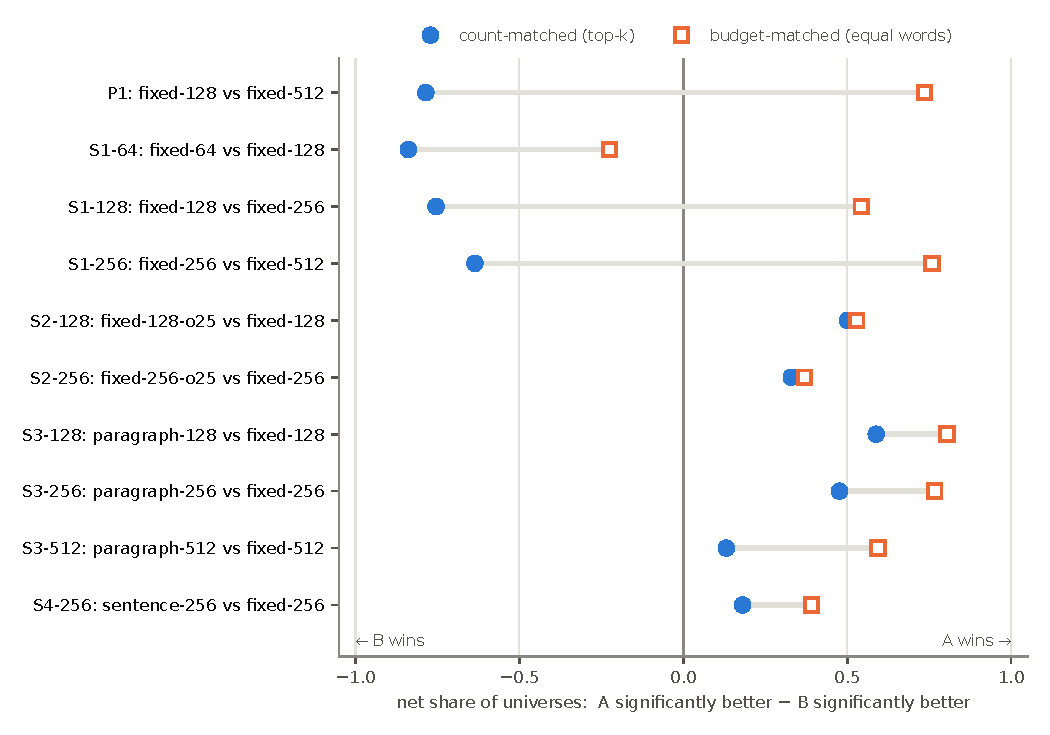
\includegraphics[width=0.94\linewidth]{figures/verdict_dumbbell.pdf}
\caption{Study 1 net support shares, $s_P(A)-s_P(B)$, for selected contrasts on the confirmatory split. Circles show count matching; open squares show word-budget matching. Movement to the right favors A relative to B, but need not reverse the favored arm.}
\label{fig:study1}
\end{figure}
% Generated by manuscript/make_tables.py from logged results. Do not edit by hand.
\begin{table*}[t]\centering\footnotesize
\caption{Study~1: share of universes (\%) whose 95\% paired interval supports arm A or arm B, per claim and selection protocol (confirmatory split); the remainder is inconclusive. Budget-matched universes use the admissible budgets $B \ge$ the larger chunk size. $n$ = number of universes.}\label{tab:e1claims}
\begin{tabular}{@{}lllrrrrrr@{}}\toprule
Claim & Role & A vs B & A (count) & B (count) & $n$ & A (budget) & B (budget) & $n$\\\midrule
P1 & primary & \texttt{fixed-128} vs \texttt{fixed-512} & 0.0 & 78.5 & 768 & 81.2 & 7.6 & 576\\
\midrule
S1-64 & secondary & \texttt{fixed-64} vs \texttt{fixed-128} & 0.0 & 83.9 & 768 & 20.0 & 42.5 & 960\\
S1-128 & secondary & \texttt{fixed-128} vs \texttt{fixed-256} & 0.0 & 75.4 & 768 & 60.8 & 6.5 & 768\\
S1-256 & secondary & \texttt{fixed-256} vs \texttt{fixed-512} & 0.0 & 63.5 & 768 & 78.0 & 2.1 & 576\\
\midrule
S2-64 & secondary & \texttt{fixed-64-o25} vs \texttt{fixed-64} & 52.5 & 1.7 & 768 & 55.3 & 1.7 & 960\\
S2-128 & secondary & \texttt{fixed-128-o25} vs \texttt{fixed-128} & 52.0 & 1.8 & 768 & 54.8 & 1.9 & 960\\
S2-256 & secondary & \texttt{fixed-256-o25} vs \texttt{fixed-256} & 36.2 & 3.3 & 768 & 39.8 & 2.9 & 768\\
S2-512 & secondary & \texttt{fixed-512-o25} vs \texttt{fixed-512} & 9.6 & 8.3 & 768 & 12.0 & 7.1 & 576\\
\midrule
S3-64 & secondary & \texttt{paragraph-64} vs \texttt{fixed-64} & 62.2 & 5.7 & 768 & 75.7 & 0.0 & 960\\
S3-128 & secondary & \texttt{paragraph-128} vs \texttt{fixed-128} & 60.0 & 1.2 & 768 & 80.4 & 0.0 & 960\\
S3-256 & secondary & \texttt{paragraph-256} vs \texttt{fixed-256} & 50.1 & 2.5 & 768 & 77.2 & 0.5 & 768\\
S3-512 & secondary & \texttt{paragraph-512} vs \texttt{fixed-512} & 14.7 & 1.6 & 768 & 60.9 & 1.6 & 576\\
\midrule
S4-64 & exploratory & \texttt{sentence-64} vs \texttt{fixed-64} & 58.9 & 6.1 & 768 & 69.4 & 0.3 & 960\\
S4-128 & exploratory & \texttt{sentence-128} vs \texttt{fixed-128} & 49.9 & 0.9 & 768 & 58.2 & 0.0 & 960\\
S4-256 & exploratory & \texttt{sentence-256} vs \texttt{fixed-256} & 19.4 & 1.3 & 768 & 39.1 & 0.0 & 768\\
S4-512 & exploratory & \texttt{sentence-512} vs \texttt{fixed-512} & 6.4 & 0.5 & 768 & 21.4 & 0.3 & 576\\
\bottomrule\end{tabular}
\end{table*}


The decline persists in all five sensitivity analyses: \SensBHEst\pp{} with multiplicity adjustment, \SensNoSquadEst\pp{} without SQuAD, \SensDefRetEst\pp{} with the default retriever, \SensClusterEst\pp{} with document resampling, and \SensAllBudgetsEst\pp{} with all budgets (Table~\ref{tab:e1sens}). A post-hoc breakdown by metric gives declines of \HOneStrictDecline, \HOneLenientDecline{} and \HOneCoverageDecline\pp{} for strict containment, lenient hits and coverage, so H1 does not rest on one metric. The direction of the budget-matched comparison does depend on the metric when gold spans are long. Qasper's gold evidence consists of whole paragraphs (median shortest span \GoldMedianQasper{} words), and there strict containment favors the 512-word arm in \QasperStrictBudgetFiveTwelve\% of budget-matched universes and the 128-word arm in \QasperStrictBudgetOneTwoEight\%, the reverse of the lenient and coverage verdicts: a 128-word window often cannot hold a whole paragraph.

The mean P1 difference changes sign between protocols in each dataset (Table~\ref{tab:e1bydataset}). The strength of the change is not uniform. CUAD has relatively few decisive count-matched settings. Qasper has mixed budget-matched verdicts and only a small positive average difference. The coverage curves in Figure~\ref{fig:p1curve} show this variation rather than reducing it to a single pooled preference.
\begin{figure}[htbp]
\centering
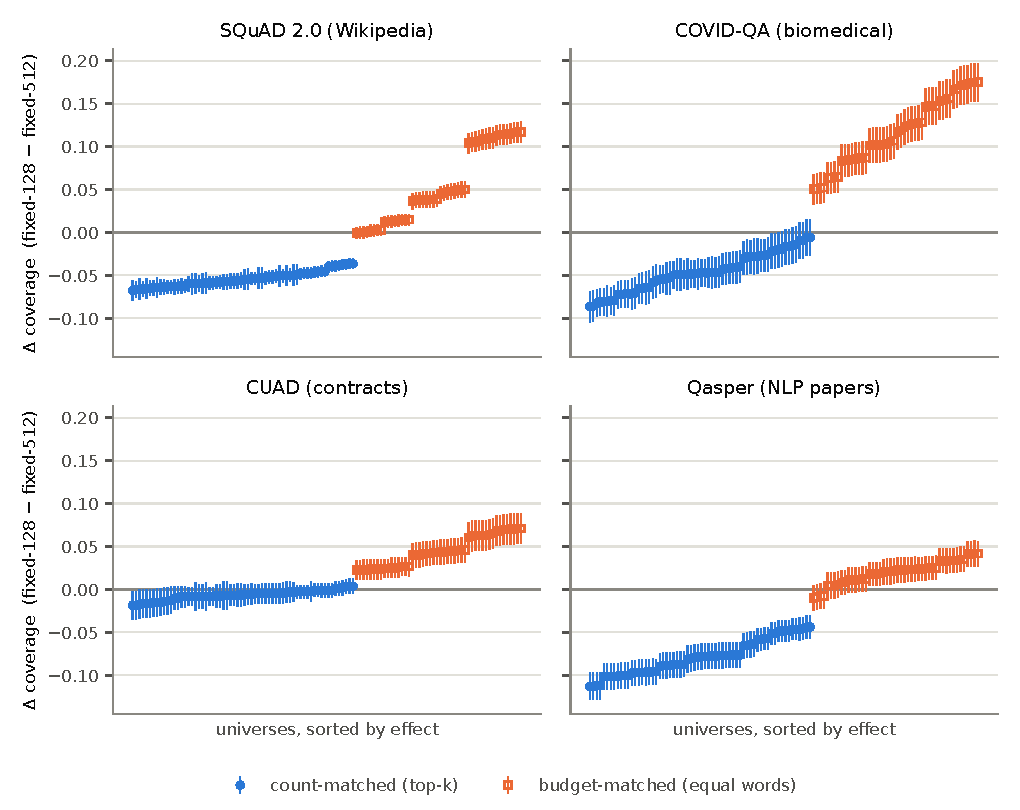
\includegraphics[width=\linewidth]{figures/speccurve_P1_coverage.pdf}
\caption{P1 coverage differences: \chunk{fixed-128} minus \chunk{fixed-512}, with 95\% Wald intervals (query level). Universes are sorted by effect within each dataset and distinguished by selection protocol.}
\label{fig:p1curve}
\end{figure}

\paragraph{Overlap, structure and size.}
Overlap comparisons change much less. For S2-128, overlap support moves from \StwoOneTwoEightCountA\% to \StwoOneTwoEightBudgetA\%; for S2-256, from \StwoTwoFiveSixCountA\% to \StwoTwoFiveSixBudgetA\%. These arms share a nominal cap, though terminal fragments produce slightly different mean lengths and overlap changes redundancy. Their relative stability is consistent with the text-allowance explanation but does not isolate it from other properties of the retrieved context.

For S3-256, paragraph-packing support rises by \HOneBEst\pp{} (95\% CI [\HOneBLo, \HOneBHi]); H1b is \HOneBVerdict. Paragraph packing produces shorter chunks on average than fixed windows at the same cap. Budget matching removes the unequal allowance in word occurrences, while leaving differences in boundaries and ranking intact. The effect is not uniform across domains (Figure~\ref{fig:s3curve}).

Part of the paragraph advantage may come from how the datasets are built. Our documents join each dataset's own contexts or paragraphs with blank lines, and paragraph packing splits exactly there, so it rarely cuts a gold span. In a post-hoc count at a 256-word cap, at least one gold span lies inside a single chunk for \ContainParagraphQasper\% of Qasper queries under paragraph packing, against \ContainFixedQasper\% for fixed windows (CUAD: \ContainParagraphCuad\% and \ContainFixedCuad\%); sentence packing reaches \ContainSentenceQasper\% on Qasper. The advantage is concentrated where fixed windows split the evidence: under budget matching, the mean Qasper S3-256 difference over all budget-matched universes (all metrics) is \QasperSplitDelta{} for the \QasperSplitShare\% of queries whose evidence \chunk{fixed-256} splits, and \QasperContainedDelta{} for the others. An advantage remains where both chunkings contain the evidence (in SQuAD, where fixed windows split the evidence of only \SquadSplitN{} queries, the mean difference among the others is \SquadContainedDelta), and the two groups of queries also differ in evidence length. Boundary alignment is therefore a plausible partial explanation, not an established cause, and the S3 contrasts should not be read as a general advantage of structure-aware chunking.

Smaller is not always better under budget matching. In S1-64, the 128-word arm retains \SoneSixFourBudgetB\% support, compared with \SoneSixFourBudgetA\% for the 64-word arm. The result is protocol dependence, not a rule to choose the smallest available chunk.

\paragraph{Dataset dependence and power.}
For S3-256 under budget matching, dataset has $\eta^2=\HTwoDatasetEta$, followed by budget and then the retriever ($\eta^2=\HTwoRetrieverEta$), and is the largest factor in \HTwoFraction\% of bootstrap replicates (\HTwoDocFraction\% with documents as the unit). H2 is \HTwoVerdict; the more precise decomposition is in Table~\ref{tab:e1h2}. Given the alignment effect above, a large dataset term is expected.

Across S2/S3 budget-matched universes, \HThreeShare\% have an estimated requirement above 500 paired queries, with median \HThreeMedianN{} (Table~\ref{tab:e1h3}). H3 is \HThreeVerdict. These estimates describe the observed paired-difference variance under the planning assumptions, not guaranteed power for a new document-clustered sample.
\section{Study 1b: semantic chunking and dense retrieval}\label{sec:study1b}
\subsection{Design}
Study 1b extends the configurations while retaining the datasets, confirmatory queries, metrics and analysis procedure. It is not an independent replication on new data. Its own written plan (version 1.0) specifies the hypotheses and analysis.

\paragraph{Semantic chunkers.}
The \chunk{semantic-bp} arm embeds sentences individually and inserts a boundary when the cosine distance between adjacent sentences exceeds the document's 95th percentile, calculated with linear interpolation. A one-sentence document becomes one chunk. Overlong sentences are split first; groups exceeding 512 words are repacked with the sentence rule. The percentile is fixed in our design rather than attributed to Qu et al.'s evaluated settings.

The \chunk{semantic-cl} arm uses the positional--semantic distance introduced by Qu et al.~\cite{qu2025semanticchunking}:
\begin{align}
d(i,j)&=\lambda d_{\mathrm{pos}}(i,j)+(1-\lambda)d_{\mathrm{cos}}(i,j),\\
d_{\mathrm{pos}}(i,j)&=|i-j|/n,\qquad d_{\mathrm{cos}}(i,j)=1-\max\{\cos(e_i,e_j),0\}.
\end{align}
Here $n$ is the number of sentences and $e_i$ is a sentence embedding. We set $\lambda=0.5$, visit pairs with $d\leq0.5$ in increasing-distance order, break ties by sentence indices, and merge clusters only while their combined length remains at most 512 words. The resulting text can be non-contiguous; intervals are concatenated in document order. Qu et al.\ also stop merging at distance 0.5, but cap clusters by a number of sentences derived from the target number of chunks; the word cap makes this an adaptation of their procedure.

Both semantic chunkers embed sentences with BGE-M3, the dense retriever's encoder. We compare each with \chunk{fixed-128}, \chunk{fixed-256} and \chunk{fixed-512}, denoting breakpoint contrasts S5 and clustering contrasts S6. Breakpoint chunks average \SemBpMin--\SemBpMax{} words across datasets, while clustering chunks average \SemClMin--\SemClMax{}. At least \SemClNoncontigMin\% of clustering chunks are non-contiguous (Table~\ref{tab:chunklen}). This setting produces clusters near the cap, so the results need not generalize to other clustering configurations.

\paragraph{Retrieval and hypotheses.}
We use default BM25 and BGE-M3 dense retrieval~\cite{chen2024bgem3}. Dense embeddings are normalized, stored in half precision and ranked by their dot product, which equals cosine similarity up to half-precision rounding. The maximum encoder input is 8,192 tokens. Word caps and token counts are different quantities, so the cap alone is not a check for encoder truncation.

For each dataset and contrast, the shorter arm is determined from corpus-average chunk lengths, a property of the chunking alone (Table~\ref{tab:chunklen}). The breakpoint arm is longer than the 128- and 256-word fixed arms and shorter than the 512-word arm. Admissible budgets are 512, 1,024 and 2,048 words. Each S5/S6 contrast has \SfiveUniversesCount{} count-matched and \SfiveUniversesBudget{} budget-matched universes; dense-only P1 has \PoneDenseUniversesCount{} and \PoneDenseUniversesBudget{}, respectively.

H4 predicts a shorter-arm support gain of at least 20 percentage points across breakpoint contrasts and retrievers. H4b uses a 10-point threshold for clustering. H5 retains H1's larger-arm formulation under dense retrieval: a decline of at least 20 percentage points in support for \chunk{fixed-512}. H4 is the single primary hypothesis of Study 1b; H4b, H5 and H5b are secondary.

In the exploratory pilot, the larger arm was already infrequently supported with dense retrieval (\HFivePilotCountFiveTwelve\% of count-matched universes), limiting how far its share could fall, while support for the shorter arm rose from \HFiveBPilotCount\% to \HFiveBPilotBudget\%. The plan's deviation log records H5b as an amendment made in response: an increase of at least 20 percentage points in support for the shorter arm. H5b was therefore formulated after its effect had been observed on the exploratory split. Its confirmatory test uses different queries over the same indexed corpus, so it is weaker evidence than H4 and H4b. H5 remains the original test.

\subsection{Results}
Across breakpoint comparisons, shorter-arm support rises from \HFourCount\% to \HFourBudget\%, a gain of \HFourEst\pp{} (95\% CI [\HFourLo, \HFourHi]). H4 is \HFourVerdict. The gain remains when retrievers are examined separately: \HFourBmOnlyEst\pp{} for BM25 and \HFourDenseOnlyEst\pp{} for dense retrieval. Table~\ref{tab:e3sens} reports the sensitivity analyses, and Figure~\ref{fig:study1b} shows the net shares of every Study 1b contrast.

These shorter-arm shares should not be read as semantic-arm shares. Against \chunk{fixed-128}, the breakpoint arm is supported in \SfiveOneTwoEightCountSem\% of count-matched universes but only \SfiveOneTwoEightBudgetSem\% of budget-matched universes. Against \chunk{fixed-512}, where the breakpoint arm is shorter, its support increases instead (Table~\ref{tab:e3claims}). Relative length changes the interpretation of the same semantic-versus-fixed comparison.
\begin{figure}[htbp]
\centering
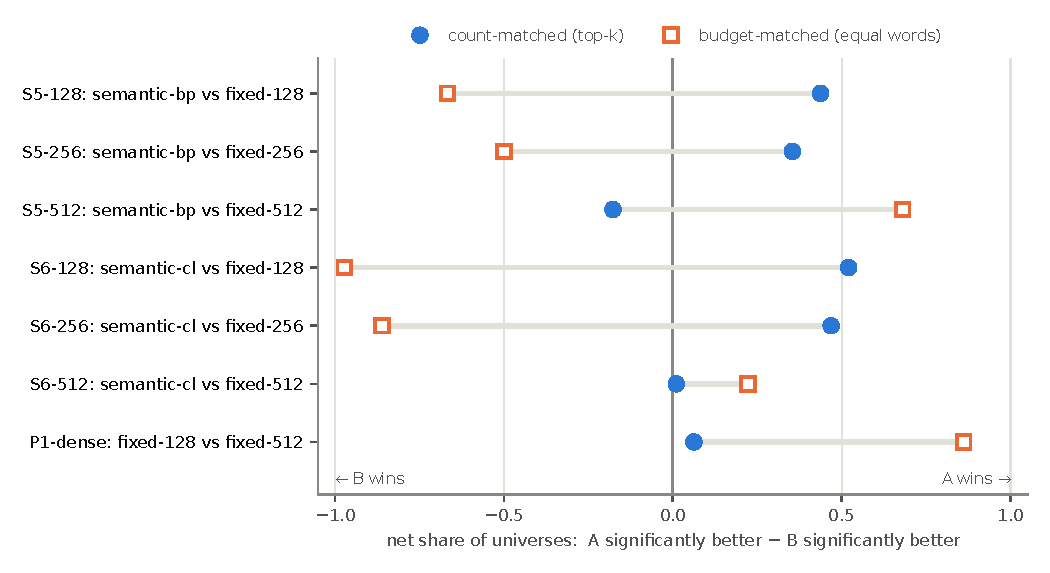
\includegraphics[width=0.95\linewidth]{figures/study1b_dumbbell.pdf}
\caption{Study 1b net support shares. S5/S6 pool default BM25 and dense retrieval; P1-dense uses only BGE-M3. A and B remain fixed within each row, so movement must be read alongside the pair's relative lengths.}
\label{fig:study1b}
\end{figure}
% Generated by manuscript/make_tables.py from logged results. Do not edit by hand.
\begin{table}[t]\centering\footnotesize
\caption{Study~1b: share of universes (\%) supporting arm A or B per claim and protocol (confirmatory). S5/S6 pool BM25 and dense retrieval; P1-dense uses the dense retriever only. Admissible budgets $B \in \{512, 1{,}024, 2{,}048\}$. The S5/S6 rows give semantic-arm (not shorter-arm) shares, the analogue of the semantic-versus-fixed comparisons in semantic-chunking studies (planned descriptive analysis g).}\label{tab:e3claims}
\begin{tabular}{@{}llrrrrrr@{}}\toprule
Claim & A vs B & A (count) & B (count) & $n$ & A (budget) & B (budget) & $n$\\\midrule
S5-128 & \texttt{semantic-bp} vs \texttt{fixed-128} & 60.4 & 16.7 & 96 & 8.3 & 75.0 & 72\\
S5-256 & \texttt{semantic-bp} vs \texttt{fixed-256} & 39.6 & 4.2 & 96 & 2.8 & 52.8 & 72\\
S5-512 & \texttt{semantic-bp} vs \texttt{fixed-512} & 8.3 & 26.0 & 96 & 68.1 & 0.0 & 72\\
\midrule
S6-128 & \texttt{semantic-cl} vs \texttt{fixed-128} & 54.2 & 2.1 & 96 & 0.0 & 97.2 & 72\\
S6-256 & \texttt{semantic-cl} vs \texttt{fixed-256} & 46.9 & 0.0 & 96 & 0.0 & 86.1 & 72\\
S6-512 & \texttt{semantic-cl} vs \texttt{fixed-512} & 18.8 & 17.7 & 96 & 33.3 & 11.1 & 72\\
\midrule
P1-dense & \texttt{fixed-128} vs \texttt{fixed-512} & 33.3 & 27.1 & 48 & 91.7 & 5.6 & 36\\
\bottomrule\end{tabular}
\end{table}


For clustering, shorter-arm support rises from \HFourBCount\% to \HFourBBudget\%, a gain of \HFourBEst\pp{} (95\% CI [\HFourBLo, \HFourBHi]). H4b is \HFourBVerdict{} for this configuration. The comparison does not separately identify effects of length, clustering and non-contiguity.

For dense P1, larger-arm support falls from \HFiveCountFiveTwelve\% to \HFiveBudgetFiveTwelve\%. The decline of \HFiveEst\pp{} (95\% CI [\HFiveLo, \HFiveHi]) meets the support rule, but only just. The dense P1 grid has \PoneDenseUniversesCount{} count-matched and \PoneDenseUniversesBudget{} budget-matched universes, so one count-matched verdict moves the share by \PoneDenseOneUniverse{} percentage points, more than the margin above the threshold. With documents as the unit, the decline is \HFiveDocEst\pp{} ([\HFiveDocLo, \HFiveDocHi]) and H5 is \HFiveDocVerdict; under the plans' computation it was \HFivePlannedEst\pp{} and \HFivePlannedVerdict. The difference between the computations comes from a single SQuAD universe whose percentile interval ends exactly at zero. The interval runs from below the threshold to well above it, and its replicates average \HFiveReplicateOffset{} points more than the estimate. We therefore treat H5 as unresolved, neither supported nor evidence against the hypothesis. The amended shorter-arm share rises from \HFiveBCount\% to \HFiveBBudget\%, a gain of \HFiveBEst\pp{} ([\HFiveBLo, \HFiveBHi]; with documents as the unit \HFiveBDocEst\pp, [\HFiveBDocLo, \HFiveBDocHi]); H5b is \HFiveBVerdict{} at both units. The floor that motivated the amendment was less severe in the confirmatory data: the larger arm's count-matched support was \HFiveCountFiveTwelve\%, against \HFivePilotCountFiveTwelve\% in the pilot.

Table~\ref{tab:h} summarizes the eight planned hypotheses. For each supported share hypothesis other than H5 (H1, H1b, H4, H4b and H5b), the lower bound of the interval also exceeds the threshold, at both units.
\begin{table*}[tb]\centering\footnotesize
\caption{Planned hypotheses and confirmatory outcomes, with queries (the planned unit) and with documents as the sampling unit. Share changes are percentage points, not retrieval-score improvements. H5b is a disclosed amendment formulated after the pilot. Table~\ref{tab:inference} adds the plans' original computation.}\label{tab:h}
\begin{tabular}{@{}llllll@{}}\toprule
ID & Role & Quantity & Estimate [95\% CI] or diagnostic & Verdict & Document unit\\\midrule
H1 & primary & Larger-arm decline, P1 & \HOneEst\pp{} [\HOneLo, \HOneHi] & \HOneVerdict & \HOneDocEst\pp{} [\HOneDocLo, \HOneDocHi], \HOneDocVerdict\\
H1b & secondary & Paragraph-256 gain & \HOneBEst\pp{} [\HOneBLo, \HOneBHi] & \HOneBVerdict & \HOneBDocEst\pp{} [\HOneBDocLo, \HOneBDocHi], \HOneBDocVerdict\\
H2 & secondary & Dataset main effect & $\eta^2=\HTwoDatasetEta$, largest in \HTwoFraction\% & \HTwoVerdict & largest in \HTwoDocFraction\%, \HTwoDocVerdict\\
H3 & secondary & Universes needing $n>500$ & \HThreeShare\%, median $n=\mbox{\HThreeMedianN}$ & \HThreeVerdict & not applicable\\\midrule
H4 & primary & Shorter-arm gain, breakpoint & \HFourEst\pp{} [\HFourLo, \HFourHi] & \HFourVerdict & \HFourDocEst\pp{} [\HFourDocLo, \HFourDocHi], \HFourDocVerdict\\
H4b & secondary & Shorter-arm gain, clustering & \HFourBEst\pp{} [\HFourBLo, \HFourBHi] & \HFourBVerdict & \HFourBDocEst\pp{} [\HFourBDocLo, \HFourBDocHi], \HFourBDocVerdict\\
H5 & secondary & Larger-arm decline, dense P1 & \HFiveEst\pp{} [\HFiveLo, \HFiveHi] & \HFiveVerdict{} (marginal) & \HFiveDocEst\pp{} [\HFiveDocLo, \HFiveDocHi], \HFiveDocVerdict\\
H5b & amendment & Shorter-arm gain, dense P1 & \HFiveBEst\pp{} [\HFiveBLo, \HFiveBHi] & \HFiveBVerdict & \HFiveBDocEst\pp{} [\HFiveBDocLo, \HFiveBDocHi], \HFiveBDocVerdict\\\bottomrule
\end{tabular}
\end{table*}

\section{Exploratory answer-quality evaluation}\label{sec:tier2}
\subsection{Setup}
We sampled 50 confirmatory queries per dataset using seed 20261019 and evaluated P1 and S3-256 with default BM25. The operating points were top-5 retrieval and a 1,024-word budget. A written generation analysis plan specifies the sample, the operating points and the analysis; the check is exploratory and does not change any confirmatory hypothesis verdict.

The reader is Qwen3-4B~\cite{qwen2025qwen3}, using a Q4\_K\_M quantized GGUF model with greedy decoding, thinking disabled and a 256-token output limit. The prompt gives numbered passages and the question, requesting the shortest supported answer or exactly ``unanswerable''. We score answers by SQuAD-style token F1 and exact match against each question's gold answer strings: answer spans for SQuAD and COVID-QA, clause spans for CUAD, and Qasper's extractive, free-form or yes/no answers. Model and prompt details are in Appendix~\ref{app:impl}.

For each query, let $\Delta_q(o)$ be the answer-score difference between A and B at operating point $o$. The difference-in-differences (DiD) is
\begin{equation}
\mathrm{DiD}_q=\Delta_q(B=1{,}024)-\Delta_q(k=5).
\label{eq:did}
\end{equation}
A positive DiD means that A gains relative to B when the protocol changes; it need not mean A has the higher score at either operating point. The pooled estimate weights datasets equally and uses 2,000 stratified bootstrap resamples. We compute the same contrast for retrieval coverage and report minimum detectable effects, $\mathrm{MDE}=(1.96+0.8416)\,\mathrm{SD}/\sqrt{n}$, with SD the standard deviation of the per-query DiD over the $n=200$ queries.

\subsection{Results}
All scheduled generations completed. Coverage DiD is \EtwoPoneCov{} (95\% CI [\EtwoPoneCovLo, \EtwoPoneCovHi]) for P1 and \EtwoSthreeCov{} ([\EtwoSthreeCovLo, \EtwoSthreeCovHi]) for S3-256. Both contrasts are positive, consistent with the retrieval studies.

Answer F1 does not show a detectable positive interaction. The pooled DiDs are \EtwoPoneFone{} ([\EtwoPoneFoneLo, \EtwoPoneFoneHi]) and \EtwoSthreeFone{} ([\EtwoSthreeFoneLo, \EtwoSthreeFoneHi]); both intervals include zero, so the sign of the answer-F1 interaction is unresolved, and the data do not establish that the protocol has no effect on answers. The intervals do exclude interactions as large as the minimum detectable effects (\EtwoPoneFoneMde{} and \EtwoSthreeFoneMde{}) in either direction.

For P1, exact match moves in the opposite direction: \EtwoPoneEm{} ([\EtwoPoneEmLo, \EtwoPoneEmHi]). The pooled cell means show the 128-word arm ahead at top-5 (\EtwoEmOneTwoEightCount{} versus \EtwoEmFiveTwelveCount), but the 512-word arm ahead at the matched budget (\EtwoEmFiveTwelveBudget{} versus \EtwoEmOneTwoEightBudget). These cell means are descriptive and have no separately reported intervals. Table~\ref{tab:e2did} gives the full contrasts.
% Generated by manuscript/make_tables.py from logged results. Do not edit by hand.
\begin{table*}[t]\centering\footnotesize
\caption{Answer-quality check (exploratory; written analysis plan): difference-in-differences DiD $= \Delta(B{=}1{,}024) - \Delta(k{=}5)$, $\Delta$ = metric(A) $-$ metric(B), with 95\% bootstrap CIs (2{,}000 resamples; pooled: stratified by dataset). The retrieval mechanism predicts DiD $> 0$; an interval that includes 0 does not establish the absence of an effect. 50 queries per dataset; reader Qwen3-4B (Q4\_K\_M, greedy).}\label{tab:e2did}
\begin{tabular}{@{}llrrr@{}}\toprule
Claim & Dataset & Answer F1 & Exact match & Coverage\\\midrule
P1 & SQuAD 2.0 & $-$0.122 [$-$0.245, +0.009] & $-$0.160 [$-$0.300, 0.000] & +0.120 [+0.040, +0.220]\\
 & COVID-QA & $-$0.006 [$-$0.101, +0.090] & $-$0.060 [$-$0.160, +0.020] & +0.110 [+0.040, +0.200]\\
 & CUAD & $-$0.001 [$-$0.031, +0.033] & 0.000 [0.000, 0.000] & +0.020 [0.000, +0.060]\\
 & Qasper & +0.060 [$-$0.015, +0.158] & 0.000 [$-$0.060, +0.060] & +0.106 [+0.020, +0.214]\\
 & Pooled (stratified) & $-$0.017 [$-$0.065, +0.033] & $-$0.055 [$-$0.100, $-$0.010] & +0.089 [+0.050, +0.132]\\
 & Minimum detectable effect & 0.068 & 0.066 & 0.059\\
\midrule
S3-256 & SQuAD 2.0 & $-$0.027 [$-$0.104, +0.049] & $-$0.060 [$-$0.160, +0.060] & +0.060 [0.000, +0.140]\\
 & COVID-QA & +0.005 [$-$0.050, +0.066] & $-$0.020 [$-$0.100, +0.040] & +0.060 [0.000, +0.140]\\
 & CUAD & $-$0.008 [$-$0.027, +0.012] & 0.000 [0.000, 0.000] & 0.000 [0.000, 0.000]\\
 & Qasper & +0.045 [$-$0.017, +0.117] & +0.020 [0.000, +0.060] & +0.020 [0.000, +0.060]\\
 & Pooled (stratified) & +0.004 [$-$0.024, +0.036] & $-$0.015 [$-$0.050, +0.020] & +0.035 [+0.015, +0.060]\\
 & Minimum detectable effect & 0.044 & 0.051 & 0.036\\
\bottomrule\end{tabular}
\end{table*}


The P1 F1 MDE is \EtwoPoneFoneMde{} (computed from the standard deviation of all 200 queries; the MDE of the equal-weight estimand is \EtwoPoneFoneMdeStrat{}, a post-hoc check). An MDE describes statistical sensitivity under a power calculation; it is not an observed bound that excludes larger effects. The confidence intervals are the basis for interpreting this experiment.

Output length also matters. Of the \EtwoJobsCuad{} CUAD outputs, \EtwoTruncCuad{} reached the generation cap, as did \EtwoTruncQasper{} of the \EtwoJobsQasper{} Qasper outputs (Table~\ref{tab:e2diag}). A truncated output cannot match exactly, and the cap was reached more often in some cells than in others. In a post-hoc check, removing the \EtwoTruncQueriesCuad{} CUAD and \EtwoTruncQueriesQasper{} Qasper queries with any truncated output leaves every reading in Table~\ref{tab:e2did} unchanged (P1 exact match \EtwoPoneEmUntrunc, [\EtwoPoneEmUntruncLo, \EtwoPoneEmUntruncHi]). So does resampling documents instead of queries (\EtwoPoneEmDoc, [\EtwoPoneEmDocLo, \EtwoPoneEmDocHi]), which matters because sampled queries share documents in SQuAD, COVID-QA and CUAD. The negative exact-match interaction comes from SQuAD (\EtwoPoneEmSquad) and COVID-QA (\EtwoPoneEmCovid); exact match is zero in every CUAD cell and rare for Qasper's free-form answers. For P1 on SQuAD at the matched budget (an exploratory observation), F1 is \EtwoSquadFiveTwelveBudgetFone{} with the longer passages and \EtwoSquadOneTwoEightBudgetFone{} with the shorter passages, at similar coverage (\EtwoSquadFiveTwelveBudgetCov{} and \EtwoSquadOneTwoEightBudgetCov{}). Passage continuity is a possible explanation, not an established mechanism.

\section{Discussion}\label{sec:discussion}
\subsection{What changes when the protocol changes?}
Count matching makes retrieval depth equal; budget matching makes the allowance in word occurrences equal. Neither holds every property of the context fixed. Longer passages may contain more evidence, but segmentation also affects ranking, redundancy, boundaries and continuity. The small overlap shifts and the direction of the unequal-length comparisons are consistent with text allowance contributing to protocol sensitivity. They do not identify it as the sole cause.

Budget matching also has costs. It can cut through the final passage, and equal word counts do not imply equal model-token counts, unique context, indexing cost or latency. These are reasons to specify the constraint, not reasons to avoid the comparison. Fixed-$k$ evaluation answers a legitimate deployment question when the system retrieves a fixed number of passages. The problem arises when its answer is presented as an intrinsic property of a chunker.

The dense retriever begins with a different preference from the lexical grid. Under count matching, it supports the 128-word arm in \HFiveBCount\% of universes and the 512-word arm in \HFiveCountFiveTwelve\%, whereas the lexical grid supports them in \PoneCountOneTwoEight\% and \PoneCountFiveTwelve\%. Topic mixing within an embedding is one possible explanation, but our experiment does not measure that mechanism. What it establishes is configuration dependence.

\subsection{Why retrieval evidence is not enough}
The answer experiment adds a distinction. Increased gold-span coverage can coexist with unresolved answer-F1 effects and an exact-match interaction in the opposite direction. A reader may respond differently to passage continuity, distractors, answer length and normalization. The present check cannot separate those explanations, and its single-reader setting does not support a general claim that protocol effects stop at retrieval.

\subsection{Reporting implications}
A chunking comparison should specify nominal caps, realized length distributions, overlap handling, retriever, metric and operating point. For the retrieved context, it should report both passage count and word or token volume, including the treatment of repeated text and the final chunk. Showing count-matched and budget-matched results side by side makes their different constraints visible.

Statistical summaries need the same precision. Support shares require universe counts, grid weights and an uncertainty procedure. They should not be called flip rates without pairing universes and measuring transitions. Query-level and document-level resampling should be distinguished, and one decision rule should define both a point estimate and its interval. Finally, retrieval and answer outcomes should be reported separately: neither substitutes for the other.

\section{Limitations and threats to validity}\label{sec:limitations}
\paragraph{Measurement.}
Our span metrics reward any qualifying or best-covered evidence span and do not penalize irrelevant context. They need not predict precision, complete multi-hop evidence acquisition, factuality or answer quality. Word budgets count repeated occurrences, whereas coverage is measured on unique word positions. The metrics are computed on words, not on characters as the plans state; a post-hoc character-based rescoring of the BM25 selections changed no hypothesis verdict, but its effect on the dense-retrieval results was not quantified. We did not evaluate precision-sensitive measures, such as token-level precision or a graded ranking metric over evidence, so we cannot say how much of the budget-matched advantage of small chunks reflects better ranking rather than more independently ranked units.

\paragraph{Implementation and scope.}
Sentence splitting is rule-based, paragraph boundaries depend on blank lines and coincide with the datasets' annotation units, and budget selection can truncate a chunk. Each query was ranked only to a fixed depth derived from corpus chunk lengths; in \UnderfillCells{} stored selections (dense retrieval, Qasper, 2,048-word budget) that prefix held \UnderfillWordsA{} and \UnderfillWordsB{} words, short of the budget, and no other stored selection fell short. Setting both selections to the maximum possible scores changes no hypothesis verdict or estimate and moves interval bounds by at most \UnderfillMaxShift{} percentage points (a post-hoc bound; the dense ranking could not be re-executed). Dense rankings use the dot product of half-precision unit vectors, so near-ties can be reordered. In 12 of the 2,202 Qasper questions, an evidence paragraph occurs twice in its paper and only the first occurrence counts as gold. Each semantic chunker uses one setting. The clustering arm is mostly non-contiguous and close to its cap. Same-cap overlap contrasts differ in realized lengths and redundancy, so they are not exact mechanistic controls. The study covers four English collections, one lexical family and one dense encoder. Study 1b reuses Study 1's confirmatory queries. The answer check uses one quantized reader, a small query sample and an output cap that truncated some responses.

\paragraph{Inference.}
Universes are correlated settings, not independent replications. A universe's verdict depends on its sample size as well as on its effect, so support shares behave like vote counts: a dataset with more queries (SQuAD, \EoneNqSquadtwo{}, against \EoneNqCuad{} for CUAD) yields decisive verdicts for smaller effects. Mean differences per dataset are in Table~\ref{tab:e1bydataset}. Joint resampling preserves their shared-query dependence but does not sample new datasets. We report query- and document-level inference; SQuAD has only 28 confirmatory documents, so its document-level intervals rest on few clusters. The per-universe intervals rely on approximate normality of mean differences, and the share intervals are approximate for the reasons given in Section~\ref{sec:study1}. Support shares depend on the grid, its weights and the significance rule. H3 uses an approximate power calculation. The answer experiment is exploratory, not a multiplicity-controlled family of confirmatory tests.

\paragraph{Study history.}
H5b was added after the pilot, and one document-bootstrap sensitivity interval was corrected after the Study 1 run; both are listed in Appendix~\ref{app:deviations}. The inference procedure was corrected after all results were known; Table~\ref{tab:inference} keeps the plans' computation alongside. The stored analysis of the Study 1 pilot predates two logged changes (sensitivity intervals from 200 rather than 1,000 joint replicates, and query resampling inside the document-cluster interval). With those settings its \PilotBounds{} affected interval bounds reproduce exactly; the current code moves them by at most \PilotMaxDiff{} percentage points and changes no estimate or verdict. The analysis plans were not deposited with an external registry, so the dates in their deviation logs are the project's own records. The post-hoc checks reported here (metric breakdown, gold-span containment, character-based metrics, the underfill bound and the answer-check sensitivity analyses) were chosen after the results were known.

\section{Conclusion}
Chunking verdicts depend on the retrieval-selection protocol. Matching words instead of chunk count reduces support for the larger fixed arm by \HOneEst\pp{} in the primary lexical comparison. In breakpoint comparisons, the shorter arm gains \HFourEst\pp{}. Both hold with documents as the sampling unit. These are changes in support shares within the evaluated grid, not universal rankings of chunkers. The original dense-retrieval hypothesis is unresolved, because its verdict depends on the inference unit, while its disclosed shorter-arm amendment, formulated after the pilot, is supported at both units.

The answer-quality check does not detect a corresponding positive F1 interaction, although its intervals exclude interactions as large as its minimum detectable effects; for the primary comparison, exact match moves in the opposite direction. The practical lesson is to state what the comparison holds constant: report retrieval depth and text budget, and test answer quality rather than infer it from evidence coverage.

\section{Reproducibility}\label{sec:reproducibility}
The code, the analysis plans with their deviation logs, dataset manifests with SHA-256 digests of the source files, run configurations, per-query results and analysis outputs accompany this paper. Every result value in the text, tables and figures is generated from the stored result files, and a separate script recomputes each reported value from its source; design constants (dataset names, grid sizes, seeds, thresholds) are written directly in the text.

Recomputing an analysis from stored outputs is not the same as re-running an experiment. From the stored per-query results, the planned analyses of the confirmatory runs and of the answer check recompute without difference, the stored pilot analysis recomputes except for the \PilotBounds{} interval bounds described in Section~\ref{sec:limitations}, and the reported analyses were also reproduced by an independent implementation of the verdict rule and the resampling. Of the experiments, only BM25 retrieval was re-executed from the public data; it reproduced every stored score and word count. Dense retrieval and answer generation need a GPU and were not re-executed; half-precision embeddings and greedy decoding can differ across hardware. The stored runs predate the run format that records digests of the code and inputs.

\section*{Use of generative AI tools}
The author designed the study, wrote the core experimental pipeline (chunking, retrieval, evaluation, semantic chunking, dense retrieval, generation and run code), made the methodological and experimental decisions, ran the experiments, read the cited literature and interpreted the results. An AI assistant (Claude, Anthropic) was used under the author's direction to help draft the Study 1b analysis plan, run literature searches, debug and revise parts of the code, implement parts of the statistical-analysis, validation and test code, draft and revise manuscript text, and check the reported computations. The author reviewed all AI-produced code and text and takes full responsibility for the content of the paper.

\FloatBarrier
\bibliographystyle{plainnat}
\bibliography{refs}

\appendix
\section{Deviations from the analysis plans}\label{app:deviations}
Table~\ref{tab:deviations} summarizes the changes logged in the two plans' deviation logs and the differences between the plans' text and the implementation. The timing column reports what the logs record. H5b adds a secondary hypothesis without replacing H5. The post-run Study 1 correction changes the document-cluster sensitivity interval, not its point estimate or verdict. The inference correction changes estimates by at most \InferenceShiftMax{} percentage points and only H5's verdict (Table~\ref{tab:inference}). Section-number errors in the plans' cross-references are listed in a separate erratum. Two exploratory items in the plans are not reported: the chunk-level reciprocal rank RR@10 of Study 1 (stored with the results) and an optional answer check for S5-256 in Study 1b, which was not run.
\begin{table}[htbp]\centering\footnotesize
\caption{Study-plan deviations (as logged) and differences between the plans' text and the implementation.}\label{tab:deviations}
\begin{tabular}{@{}>{\raggedright\arraybackslash}p{1.55cm}>{\raggedright\arraybackslash}p{5.5cm}>{\raggedright\arraybackslash}p{7.4cm}@{}}\toprule
Study & Change & Timing as logged, and consequence\\\midrule
Study 1 & Restrict main budgets to $B\geq\max(W_A,W_B)$; retain all budgets for sensitivity analysis & Before the pilot and confirmatory run; a smoke test showed that smaller budgets force truncation of the first chunk.\\
Study 1 & Add document-cluster resampling & Before the runs; multiple queries are nested in a small number of SQuAD articles.\\
Study 1 & Align the $\eta^2$ description with the analytic implementation & After the pilot and before the plan's final version; the estimand and thresholds are unchanged.\\
Study 1 & Correct query-level resampling inside the document-cluster sensitivity interval & After the confirmatory run; the interval changes, while the point estimate and verdict do not.\\
Answer check & Planned: two hosted readers, 200 queries per dataset, $k\in\{3,5\}$ and $B\in\{512,1{,}024\}$, two samples per query. Executed: one local reader (Qwen3-4B, greedy), 50 queries per dataset, $k=5$ and $B=1{,}024$ & Before any analyzed generation, following API-quota limits; the smaller sample lowers power, and the check remains exploratory.\\
Answer check & Two partial runs (21 hosted-model rows; 198 rows of a CPU run) were stopped and are not analyzed; the analyzed run is the first complete GPU run & Before the analyzed run, by the rule recorded in the log; CPU and GPU outputs are never pooled.\\
Study 1b & Specify implementation details & During implementation, before pilot output.\\
Study 1b & Add H5b and retain H5 & After the exploratory pilot, before the confirmatory run; a new secondary estimand is disclosed.\\
Study 1b & Retain the clustering defaults despite near-cap chunks & After the pilot; the configuration is not tuned to improve the observed outcome.\\
Study 1b & The plan names both the confirmatory and the full corpus for the chunk statistics that orient the shorter arm & The implementation uses the full corpus; both give the same shorter arm in all 24 dataset-claim cases.\\\midrule
All & The metrics are computed on word intervals (gold character spans mapped to the words they overlap), whereas the plans define them over characters & The reported results are word-based; a post-hoc character-based rescoring of re-executed BM25 selections changes no verdict (Appendix~\ref{app:charmetric}).\\
Study 1 & The Benjamini--Hochberg family is claim, protocol and dataset; the plan says ``within claim'' & Pooling over datasets gives \SensBHPooledEst\pp{} instead of \SensBHEst\pp{}.\\
Answer check & The reported MDE uses the pooled standard deviation of all queries & An MDE for the equal-weight estimand is reported alongside (post-hoc); values agree to about 0.001.\\
Study 1b & Budget-matched dense selections filled short of the budget: \UnderfillCells{} (Section~\ref{sec:limitations}) & Post-hoc bound: no verdict changes.\\\midrule
Both & Inference: one Wald verdict rule for every estimate and bootstrap replicate, at the query or the document unit, instead of percentile verdicts for the estimate and normal-approximation verdicts with the query-level SD in the replicates & After all results were known; estimates move by at most \InferenceShiftMax{} pp and only H5's verdict changes (Table~\ref{tab:inference}).\\
Study 1 & The stored pilot analysis predates two logged changes to the sensitivity intervals & \PilotBounds{} interval bounds differ from a recomputation by at most \PilotMaxDiff{} pp; estimates and verdicts are identical.\\\bottomrule
\end{tabular}
\end{table}
% Generated by manuscript/make_tables.py from logged results. Do not edit by hand.
\begin{table*}[t]\centering\footnotesize
\caption{Share hypotheses (pp, 95\% CI, verdict) under the reported procedure (one Wald verdict rule for the estimate and every bootstrap replicate, query level), the same procedure with documents as the resampling and variance unit, and the computation specified in the analysis plans (percentile-bootstrap verdicts for the estimate, normal-approximation verdicts with the query-level SD in the replicates).}\label{tab:inference}
\begin{tabular}{@{}llll@{}}\toprule
Hypothesis & Reported (query) & Document unit & Planned computation\\\midrule
H1 (P1 decline) & 70.9 [64.8, 81.9] supported & 68.9 [61.6, 80.9] supported & 71.1 [64.8, 81.9] supported\\
H1b (S3-256 gain) & 27.1 [15.4, 33.9] supported & 26.4 [15.0, 34.4] supported & 26.7 [15.4, 33.9] supported\\
H4 (breakpoint, shorter arm) & 55.6 [50.8, 63.1] supported & 59.0 [51.3, 65.0] supported & 55.4 [50.8, 63.1] supported\\
H4b (clustering, shorter arm) & 65.3 [56.5, 68.3] supported & 65.2 [55.4, 67.1] supported & 64.4 [56.5, 68.3] supported\\
H5 (dense P1 decline) & 21.5 [16.7, 41.7] supported & 19.4 [16.7, 39.6] inconclusive & 19.4 [16.7, 41.7] inconclusive\\
H5b (dense P1, shorter arm) & 58.3 [45.1, 64.6] supported & 58.3 [47.9, 75.0] supported & 58.3 [45.1, 64.6] supported\\
\bottomrule\end{tabular}
\end{table*}


\FloatBarrier
\section{Implementation details}\label{app:impl}
\paragraph{Dense retrieval.}
The dense-retrieval code pins BGE-M3 at revision \texttt{5617a9f61b02}. The Study 1b run manifests record \texttt{sentence-transformers} 6.1.0, \texttt{transformers} 5.20.1 and \texttt{torch} 2.14.1 on a CUDA device in half precision. They do not record the model revision, so the run records alone cannot confirm that the stored runs used the pinned revision. Normalized embeddings are cached in half precision and ranked by their dot product without renormalization; the rounding changes vector norms by at most about $5\times10^{-4}$, so only near-ties can be reordered. Equal scores are ordered by the lower chunk index. Half-precision embeddings should not be assumed bit-identical across hardware.

\paragraph{Reader and prompt.}
The generation code pins the reader to the Qwen3-4B GGUF Q4\_K\_M file at revision \texttt{bc640142} and checks the file's SHA-256 before loading it; the generation records report \texttt{llama-cpp-python} 0.3.36 but not the revision or the file digest. The pinned model-file SHA-256 is:
\begin{quote}\ttfamily\small
7485fe6f\allowbreak11af2943\allowbreak3bc51cab\allowbreak58009521\allowbreak f205840f\allowbreak5b4ae3a3\allowbreak2fa7f92e\allowbreak8534fdf5
\end{quote}
The ChatML prompt contains an empty thinking block. Decoding uses temperature zero, top-$k$ one, seed 7 and the 256-token cap. The system instruction is:
\begin{quote}\small
Answer the question using only the numbered passages. Reply with the shortest answer that is fully supported by the passages, copying the wording from them where possible. If the passages do not contain the answer, reply exactly: unanswerable
\end{quote}
The user message lists numbered passages, followed by the question and an answer cue. Keeping this wording fixed prevents prompt changes from being mixed into the protocol contrast.

\FloatBarrier
\section{Additional retrieval results}\label{app:retrieval}
The tables below give corpus-level chunk lengths, per-dataset results, sensitivity analyses and power calculations. Corpus mean length should be distinguished from the amount of text actually selected for a query.
% Generated by manuscript/make_tables.py from logged results. Do not edit by hand.
\begin{table}[t]\centering\small
\caption{Mean chunk length in words per chunking and dataset (full retrieval corpus), from the run manifests; they depend only on the chunking, not on any retrieval metric. These lengths define the ``shorter arm'' of every Study~1b claim. The fixed chunkings of Study~1b are the same chunks as in Study~1.}\label{tab:chunklen}
\begin{tabular}{@{}lrrrr@{}}\toprule
Chunking & SQuAD 2.0 & COVID-QA & CUAD & Qasper\\\midrule
\texttt{fixed-64} & 64 & 64 & 64 & 63\\
\texttt{fixed-128} & 126 & 126 & 127 & 126\\
\texttt{fixed-256} & 249 & 247 & 252 & 247\\
\texttt{fixed-512} & 485 & 483 & 495 & 477\\
\texttt{fixed-64-o25} & 64 & 64 & 64 & 64\\
\texttt{fixed-128-o25} & 127 & 127 & 127 & 127\\
\texttt{fixed-256-o25} & 252 & 252 & 253 & 251\\
\texttt{fixed-512-o25} & 497 & 494 & 502 & 491\\
\texttt{sentence-64} & 49 & 49 & 46 & 50\\
\texttt{sentence-128} & 111 & 111 & 98 & 113\\
\texttt{sentence-256} & 235 & 234 & 213 & 235\\
\texttt{sentence-512} & 476 & 470 & 453 & 466\\
\texttt{paragraph-64} & 46 & 45 & 41 & 42\\
\texttt{paragraph-128} & 90 & 90 & 85 & 88\\
\texttt{paragraph-256} & 187 & 179 & 174 & 199\\
\texttt{paragraph-512} & 420 & 392 & 379 & 435\\
\midrule
\texttt{semantic-bp} & 293 & 287 & 320 & 278\\
\texttt{semantic-cl} & 456 & 455 & 458 & 452\\
\quad non-contiguous chunks (\%) & 92.5 & 94.1 & 92.0 & 94.7\\
\bottomrule\end{tabular}
\end{table}

% Generated by manuscript/make_tables.py from logged results. Do not edit by hand.
\begin{table}[t]\centering\footnotesize
\caption{Study~1 per dataset: share of universes (\%) supporting arm A or B, and the mean difference $\bar\Delta = $ metric(A) $-$ metric(B) over universes. P1: A = fixed-128, B = fixed-512. S3-256: A = paragraph-256, B = fixed-256.}\label{tab:e1bydataset}
\begin{tabular}{@{}llrrrrrr@{}}\toprule
Claim & Dataset & A (count) & B (count) & $\bar\Delta$ (count) & A (budget) & B (budget) & $\bar\Delta$ (budget)\\\midrule
P1 & SQuAD 2.0 & 0.0 & 100.0 & $-$0.055 & 83.3 & 0.0 & +0.053\\
 & COVID-QA & 0.0 & 89.1 & $-$0.054 & 100.0 & 0.0 & +0.109\\
 & CUAD & 0.0 & 25.0 & $-$0.009 & 97.2 & 0.0 & +0.040\\
 & Qasper & 0.0 & 100.0 & $-$0.093 & 44.4 & 30.6 & +0.002\\
\midrule
S3-256 & SQuAD 2.0 & 69.8 & 0.0 & +0.014 & 100.0 & 0.0 & +0.034\\
 & COVID-QA & 76.6 & 0.0 & +0.028 & 100.0 & 0.0 & +0.058\\
 & CUAD & 1.0 & 9.9 & $-$0.003 & 9.4 & 2.1 & +0.002\\
 & Qasper & 53.1 & 0.0 & +0.019 & 99.5 & 0.0 & +0.030\\
\bottomrule\end{tabular}
\end{table}

% Generated by manuscript/make_tables.py from logged results. Do not edit by hand.
\begin{table}[t]\centering\small
\caption{Study~1, H1 under the planned sensitivity analyses: drop in the share of universes supporting fixed-512 from count- to budget-matched selection, in percentage points (threshold 20). (a) changes the verdict rule and has no joint-bootstrap CI.}\label{tab:e1sens}
\begin{tabular}{@{}lrl@{}}\toprule
Analysis & Estimate (pp) & 95\% CI\\\midrule
Main analysis & 70.9 & [64.8, 81.9]\\
\midrule
(a) Benjamini--Hochberg FDR 5\% within claim, protocol and dataset & 67.6 & ---\\
(b) without SQuAD 2.0 & 61.2 & [53.2, 74.8]\\
(c) default retriever only (Lucene, $k_1$=1.5, $b$=0.75, stemmed) & 70.8 & [64.6, 85.4]\\
(d) document resampling, cluster-robust intervals & 68.9 & [61.6, 80.9]\\
(e) all budgets, including $B <$ chunk size & 73.9 & [68.3, 84.8]\\
\bottomrule\end{tabular}
\end{table}

% Generated by manuscript/make_tables.py from logged results. Do not edit by hand.
\begin{table}[t]\centering\small
\caption{Study~1, H2: main-effects decomposition of $\Delta_u$ for S3-256 under budget-matched selection.}\label{tab:e1h2}
\begin{tabular}{@{}lr@{}}\toprule
Quantity & Value\\\midrule
$\eta^2$ of dataset & 0.614\\
$\eta^2$ of budget & 0.096\\
$\eta^2$ of retriever & 0.044\\
$\eta^2$ of metric & 0.032\\
dataset largest (share of bootstrap replicates) & 100.0\%\\
\bottomrule\end{tabular}
\end{table}

% Generated by manuscript/make_tables.py from logged results. Do not edit by hand.
\begin{table}[t]\centering\small
\caption{Study~1, H3: paired queries needed to detect $|\delta| = 0.02$ ($\alpha=0.05$ two-sided, power 0.8), $n = ((1.96 + 0.8416)\,\sigma_d / 0.02)^2$, per budget-matched universe.}\label{tab:e1h3}
\begin{tabular}{@{}lrr@{}}\toprule
Claim & Median $n$ & Universes with $n > 500$ (\%)\\\midrule
S2-64 & 1,175 & 82.5\\
S2-128 & 1,162 & 84.8\\
S2-256 & 1,149 & 79.7\\
S2-512 & 1,161 & 78.0\\
S3-64 & 1,498 & 92.5\\
S3-128 & 1,412 & 90.6\\
S3-256 & 1,399 & 86.2\\
S3-512 & 1,248 & 84.7\\
\midrule
All S2 and S3 universes & 1,256 & 85.4\\
\bottomrule\end{tabular}
\end{table}

% Generated by manuscript/make_tables.py from logged results. Do not edit by hand.
\begin{table}[t]\centering\small
\caption{Study~1b, H4 under the planned sensitivity analyses: share of S5 universes (\%) supporting the shorter arm under count- and budget-matched selection, and the difference (pp; threshold 20). Study~1b uses only the default BM25 configuration, so sensitivity (c), the default-retriever restriction, does not apply.}\label{tab:e3sens}
\begin{tabular}{@{}lrrrl@{}}\toprule
Analysis & Count & Budget & Difference & 95\% CI\\\midrule
Main analysis (H4) & 9.7 & 65.3 & 55.6 & [50.8, 63.1]\\
\midrule
(a) Benjamini--Hochberg FDR 5\% within claim, protocol and dataset & --- & --- & 54.3 & ---\\
(b) without SQuAD 2.0 & 7.4 & 55.6 & 48.1 & [42.7, 58.3]\\
(d) document resampling, cluster-robust intervals & 7.6 & 66.7 & 59.0 & [51.3, 65.0]\\
(e) all budgets & 9.7 & 63.3 & 53.6 & [49.7, 60.9]\\
(f) BM25 only & 0.0 & 61.1 & 61.1 & [57.2, 72.5]\\
(f) dense only & 19.4 & 69.4 & 50.0 & [39.1, 58.1]\\
\bottomrule\end{tabular}
\end{table}

\begin{figure}[htbp]
\centering
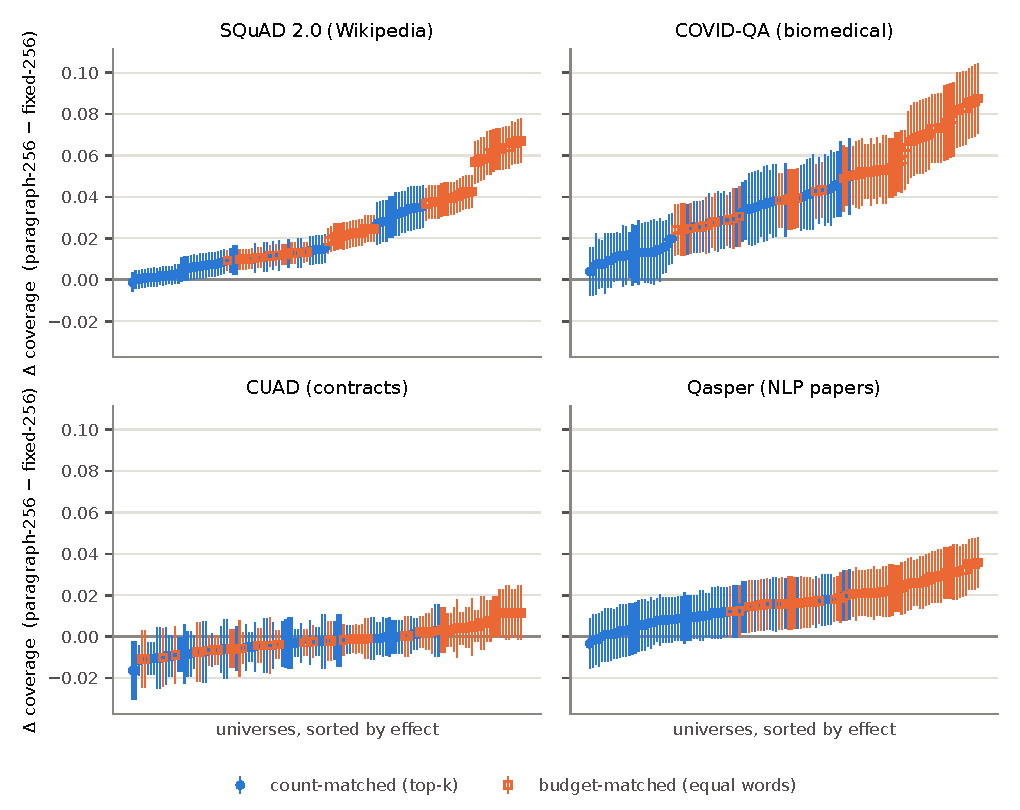
\includegraphics[width=\linewidth]{figures/speccurve_S3-256_coverage.pdf}
\caption{S3-256 coverage differences: paragraph packing minus fixed windows at a 256-word cap, with 95\% Wald intervals (query level). Universes are sorted by effect within each dataset. The near-zero CUAD effects show that the paragraph-packing result is not uniform across domains.}
\label{fig:s3curve}
\end{figure}

\FloatBarrier
\section{Post-hoc sensitivity: character-based metrics}\label{app:charmetric}
This analysis is not part of the analysis plans. Rankings and selected chunks were not stored, so BM25 retrieval was re-executed with the stored configuration. Before attributing any difference to the metric, we checked that the re-executed word scores and word counts equal the stored arrays: all \PosthocEquivElements{} stored Study 1 values and \PosthocEquivElementsB{} stored Study 1b BM25 values match exactly. Matching scores and word counts make it very likely, but do not prove, that the same chunks were selected, because the stored runs contain no chunk identifiers to compare. The re-executed selections were then scored with literal characters (whitespace between separately retrieved chunks is covered by neither chunk) and with non-whitespace characters, and analyzed with the unchanged planned analysis code and thresholds. Table~\ref{tab:charmetric} reports the result. No hypothesis verdict changes. The literal-character definition changes \PosthocCharFlips{} of \PosthocUniverses{} Study 1 universe verdicts, mostly for strict containment, and none reverses sign. Removing float16 storage changes none. The dense-retrieval arm of Study 1b was not re-executed, so the effect of the definition on H4, H4b, H5 and H5b as pooled over both retrievers is unquantified.
% Generated by manuscript/make_tables.py from logged results. Do not edit by hand.
\begin{table}[t]\centering\footnotesize
\caption{Post-hoc sensitivity (not in the analysis plans): hypothesis estimates (pp, 95\% CI) when the re-executed BM25 selections, which reproduce every stored score and word count, are scored on words (as reported), on words without float16 storage, on characters, and on non-whitespace characters. Study 1 columns: H1, H1b, H2 dataset $\eta^2$, H3 share of universes needing $n>500$, and universe verdicts that change relative to the stored scores (of 24{,}960). Study 1b rows give the H4 and H4b forms restricted to BM25 universes (the dense arm was not re-executed). All rows use the computation specified in the analysis plans, so they are compared with the planned values.}\label{tab:charmetric}
\begin{tabular}{@{}lrrrrr@{}}\toprule
Scoring & H1 / H4 (BM25) & H1b / H4b (BM25) & $\eta^2$ dataset & H3 $n>500$ (\%) & Changed verdicts\\\midrule
Stored (words, float16) & 71.1 [64.8, 81.9] & 26.7 [15.4, 33.9] & 0.614 & 85.4 & ---\\
Words, float64 & 71.1 [64.8, 81.9] & 26.7 [15.4, 33.9] & 0.614 & 85.4 & 0\\
Characters & 70.4 [63.9, 80.3] & 24.2 [13.5, 30.7] & 0.590 & 85.5 & 965\\
Non-space characters & 71.1 [64.9, 81.9] & 26.2 [15.0, 33.2] & 0.620 & 85.4 & 197\\
\midrule
Study 1b BM25: Stored (words, float16) & 61.1 [57.2, 72.5] & 63.9 [55.3, 71.1] &  &  & \\
Study 1b BM25: Words, float64 & 61.1 [57.2, 72.5] & 63.9 [55.3, 71.1] &  &  & \\
Study 1b BM25: Characters & 60.2 [54.9, 70.4] & 60.2 [52.8, 67.8] &  &  & \\
Study 1b BM25: Non-space characters & 62.0 [57.2, 72.5] & 63.9 [55.3, 71.1] &  &  & \\
\bottomrule\end{tabular}
\end{table}


\FloatBarrier
\section{Generation diagnostics}\label{app:diagnostics}
Table~\ref{tab:e2diag} summarizes completion, truncation and answer behavior over the 400 generations per dataset (50 queries, four chunkings, two operating points). The correlation is descriptive, not causal. A lenient hit means that at least half of one gold span was retrieved; it does not mean that all required evidence was present.
% Generated by manuscript/make_tables.py from logged results. Do not edit by hand.
\begin{table}[t]\centering\footnotesize
\caption{Answer-quality check, planned diagnostics per dataset (400 generations each): completed jobs, answers truncated at the 256-token cap, share of ``unanswerable'' replies, and the link between retrieval and answers (Pearson correlation of coverage and F1; mean F1 when the gold evidence was / was not at least half retrieved).}\label{tab:e2diag}
\begin{tabular}{@{}lrrrrrr@{}}\toprule
Dataset & Jobs ok & Truncated & Unanswerable (\%) & $r$(coverage, F1) & F1 | hit & F1 | miss\\\midrule
SQuAD 2.0 & 400/400 & 0 & 4.2 & 0.36 & 0.56 & 0.06\\
COVID-QA & 400/400 & 0 & 5.8 & 0.33 & 0.40 & 0.15\\
CUAD & 400/400 & 65 & 15.0 & 0.66 & 0.70 & 0.14\\
Qasper & 400/400 & 2 & 15.8 & 0.53 & 0.37 & 0.08\\
\bottomrule\end{tabular}
\end{table}


\end{document}